\documentclass[a4paper, oneside]{book}
\usepackage[italian]{babel}
\usepackage[utf8]{inputenc}
\usepackage[a4paper,top=2.5cm,bottom=2.5cm,left=2cm,right=2cm]{geometry}
\usepackage{amssymb}
\usepackage{amsthm}
\usepackage{graphics}
\usepackage{amsfonts}
\usepackage{amsmath}
\usepackage{amstext}
\usepackage{engrec}
\usepackage{rotating}
\usepackage[safe,extra]{tipa}
\usepackage{multirow}
\usepackage{hyperref}
\usepackage{enumerate}
\usepackage{braket}
\usepackage{marginnote}
\usepackage{pgfplots}
\usepackage{cancel}
\usepackage{polynom}
\usepackage{booktabs}
\usepackage{enumitem}
\usepackage{algorithm}
\usepackage{algpseudocode}
\usepackage{framed}
\usepackage{pdfpages}
\usepackage{pgfplots}
\usepackage{fancyhdr}
\usepackage{caption}
\usepackage{subcaption}
\usepackage{setspace}
\usepackage{hyperref}

\usepackage{tikz}\usetikzlibrary{er}\tikzset{multi  attribute /.style={attribute
    ,double  distance =1.5pt}}\tikzset{derived  attribute /.style={attribute
    ,dashed}}\tikzset{total /.style={double  distance =1.5pt}}\tikzset{every
  entity /.style={draw=orange , fill=orange!20}}\tikzset{every  attribute
  /.style={draw=MediumPurple1, fill=MediumPurple1!20}}\tikzset{every
  relationship /.style={draw=Chartreuse2,
    fill=Chartreuse2!20}}\newcommand{\key}[1]{\underline{#1}}
\usetikzlibrary{arrows.meta}
\usetikzlibrary{decorations.markings}
\usetikzlibrary{arrows,shapes, shapes.geometric,backgrounds,petri}
\tikzset{
  place/.style={
    circle,
    thick,
    draw=black,
    minimum size=6mm,
  },
  transition/.style={
    rectangle,
    thick,
    fill=black,
    minimum width=8mm,
    inner ysep=2pt
  },
  transitionv/.style={
    rectangle,
    thick,
    fill=black,
    minimum height=8mm,
    inner xsep=2pt
  }
}
\tikzset{elliptic state/.style={draw,ellipse}}

\usetikzlibrary{automata,positioning, calc}

\pagestyle{fancy}
\fancyhead[L,RO]{\slshape \rightmark}
\fancyfoot[C]{\thepage}

\title{Modelli della Concorrenza}
\author{Tommaso Ferrario (\href{https://github.com/TommasoFerrario18}{@TommasoFerrario18}) \\\\
Telemaco Terzi (\href{https://github.com/Tezze2001}{@Tezze2001})}
\date{October 2023}

\pgfplotsset{compat=1.13}

\begin{document}

\maketitle

\newtheorem{teorema}{Teorema}
\newtheorem{dimostrazione}{Dimostrazione}
\newtheorem{definizione}{Definizione}
\newtheorem{esempio}{Esempio}
\newtheorem{osservazione}{Osservazione}
\newtheorem{nota}{Nota}
\newtheorem{corollario}{Corollario}
\tableofcontents
\renewcommand{\chaptermark}[1]{
  \markboth{\chaptername
    \ \thechapter.\ #1}{}}
\renewcommand{\sectionmark}[1]{\markright{\thesection.\ #1}}

\chapter{Introduzione}
Possiamo definire diverse semantiche per la programmazione sequenziale:
\begin{itemize}
    \item \textbf{Operazionale}: ho una macchina astratta e definisco i vari
          passi della computazione:
          \begin{equation}
              Input \longrightarrow M \longrightarrow Output
          \end{equation}
    \item \textbf{Denotazionale}: dato un programma funzionale $P$ ho una
          funzione definita come:
          \begin{equation}
              f: \text{Dati}_{I} \to \text{Dati}_{O} \ ( \lambda-\text{calcolo})
          \end{equation}
    \item \textbf{Assiomatica}: l'input e l'output sono rappresentati come
          formule logiche. Questa tipologia prende il nome di \textit{Triple di
              Hoare}.
          \begin{equation}
              \{Input\} P \{Output\}
          \end{equation}
\end{itemize}
Nella programmazione sequenziale si hanno due punti chiave che devono essere
garantiti:
\begin{itemize}
    \item \textbf{Terminazione del programma}.
    \item \textbf{Composizionalità} tra più comandi per ottenere un programma,
          ovvero:
          \begin{equation}
              \begin{aligned}
                  s_1: x = 2 \ \ \{x = V\} \ x = 2 \ \{x = 2\} \\
                  s_2: x = 3 \ \ \{x = V\} \ x = 3 \ \{x = 3\} \\
                  \{x = V\} \ s_1; \ s_2 \ \{x = 3\}           \\
              \end{aligned}
          \end{equation}
          Se esiste un programma $s_1'$ tale che mi permette di ottenere lo
          stesso risultato si $s_1$, allora posso sostituirlo a $s_1$.
          \begin{equation}
              \begin{aligned}
                  s_1': \{x = V\} \ x = 1; \ x = x + 1  \ \{x = 2\} \\
                  \{x = V\} \ s_1'; \ s_2 \ \{x = 3\}               \\
              \end{aligned}
          \end{equation}
\end{itemize}


\chapter{Calculus of Communicating Systems}
Dati due processi $p_1$ ed $p_2$ si ha che essi sono specificati in
\textbf{esecuzione concorrente} con l'utilizzo della seguente notazione:
\begin{equation}
    p_1 | p_2 \ \text{dove} \ p_1, p_2 \in Proc_{CCS}
\end{equation}
L'esecuzione in concorrenza può portare a diverse complicanze qualora non venga
rispettato, per esempio, un certo ordine di esecuzione. Si ha quindi il
\textbf{non determinismo}, ovvero il risultato ottenuto dall'esecuzione dei
programmi dipende dall'ordine di esecuzione di essi. Inoltre, si perde la
composizionalità dei processi.
\begin{esempio}[\textbf{Non determinismo e nessuna composizionalità}]
    Supponiamo di avere due programmi $p_1$ e $p_2$ definiti nel seguente
    modo:
    \begin{equation}
        \begin{aligned}
            p_1 =\{x = V\} x = 2 \{x = 2\} \\
            p_2 =\{x = V\} x = 3 \{x = 3\}
        \end{aligned}
    \end{equation}
    con $V$ che indica un qualunque valore.

    L'esecuzione in parallelo di questi due programmi mi permette di ottenere i
    seguenti risultati:
    \begin{equation}
        \{x = V\} \ p_1 | p_2 \ \{x = 2 \lor x = 3\}
    \end{equation}
    avendo quindi una situazione di non determinismo. Inoltre, definendo un nuovo
    problema $p_1'$ possiamo osservare come la proprietà di compo<sizionalità non
    risulta più valida.
    \begin{equation}
        p_1' = \{x = V\} \ x = 1; x = x + 1 \ \{x = 2\}
    \end{equation}
    Se proviamo a sostituire questo programma al posto di $p_1$ otteniamo:
    \begin{equation}
        \{x = V\} \ p_1' | p_2 \ \{x = 2 \lor x = 3 \lor x = 4\}
    \end{equation}
\end{esempio}
Per mantenere il principio di composizionalità si cambia linguaggio di rappresentazione.
Per modellare sistemi concorrenti esistono diverse cose:
\begin{itemize}
    \item \textbf{Algebre di processi}: CCS e CSP
    \item \textbf{Automi a stati finiti}: tutti gli automi a stati finiti e i
          riconoscitori di linguaggi, ricadono anche i sistemi di transizione
          etichettati, quest'ultimi utili per modellare la semantica interleaving
          delle algebre dei processi.
    \item \textbf{Reti di petri}
\end{itemize}
\section{Algebre dei processi}
Hoare ha introdotto un nuovo paradigma di programmazione, il paradigma \textbf{CSP}
(\textit{Communicating Sequential Processes}). In questo paradigma non si ha
più una memoria condivisa, ma un insieme di processi ciascuno con una sua memoria
privata. Si ha un'interazione tra processi tramite lo scambio di messaggi del
tipo hand-shacking, avendo quindi la sincronizzazione basata sullo scambio
di informazioni. Viene fatto anche un processo particolare rappresentante la memoria
condivisa. Avremo quindi:
\begin{equation}
    x \ | \ p_1 \ | \ p_2
\end{equation}
dove $x$ che rappresenta la memoria condivisa dai due processi.

Un diverso paradigma è quello proposto da Milner, il quale propose il lambda
calcolo ($\lambda$-calcolo) per passare dal paradigma sequenziale a quello
concorrente. In questo si studia in modo approfondito la composizionalità, sfruttando
la composizione tra funzioni, cercando di non perderla nel concorrente.
Introduce quindi una sorta di $\lambda$-calcolo concorrente, introducendo il
\textbf{CCS} (\textit{Calculus of Communicating Systems}), in cui pensa ad un
calcolo algebrico per sistemi comunicanti. Adotta anche lui un paradigma che
studia un sistema formato da componenti, chiamati processi. Questi processi
comunicano tramite la sincronizzazione delle operazioni. Per la gestione di queste
si utilizza la seguente notazione:
\begin{itemize}
    \item \textbf{$a$}: indichiamo un processo generico che invia il messaggio.
    \item \textbf{$\overline{a}$}: indichiamo un processo generico che riceve.
\end{itemize}
Un \textbf{sistema}, quindi, è un insieme di processi il cui comportamento è gestito da
un calcolo algebrico, si punta alle algebre di processi, ovvero linguaggi di
specifica di sistemi concorrenti che si ispirano al calcolo dei sistemi comunicanti.

I messaggi di scambio corrispondono ad uno scambio di valori di variabili e questo
è rappresentabile dall'algebra. Utilizzando questa tecnica, i processi possono
interagire anche con l'ambiente esterno attraverso delle porte. Sfruttando
questa tecnica non si ha più un sistema chiuso.

Dato un sistema $P$, si scrive:
\begin{equation}
    P = p_1 \ | \ p_2 \ | \ p_3
\end{equation}
se $P$ è formato dai processi $p_1$, $p_2$ e $p_3$, processi che sono interagenti a
due a due. Ogni processo ha comunque una memoria privata.

Milner risolve il problema della \textit{composizionalità} tramite l'uso di diverse
porte che permettono ad un processo di comunicare con altri o con l'ambiente esterno.
Quindi ogni processo può essere visto come un insieme di sotto-processi interagenti
che però interagiscono tramite sincronizzazione con i processi esterni tramite
una porta. Bisogna comunque mantenere il comportamento complessivo. Per il
processo esterno è come se sostituissi il processo con cui comunica con il suo
sotto-processo. Si introduce il concetto di \textbf{equivalenza all'osservazione},
che permette di sostituire un processo $p_i$ con uno $p_i'$ se sono equivalenti
rispetto all'osservazione, ovvero se e solo se un qualsiasi osservatore esterno
non è in grado di distinguere i due processi.

Con il termine \textit{osservare} ci si riferisce all'interazione con il sistema
dove agisce il processo. Questo deve essere valido per ogni possibile osservatore.
Se questo è garantito la sostituzione di un processo non va a modificare
l'esecuzione complessiva, senza incorrere in deadlock o altre problematiche.
Per verificare l'equivalenza esistono diverse tecniche tra cui la \textbf{bisimulazione}.
\section{Labeled Transition System}
Per modellare la semantica interleaving delle algebre dei processi si utilizzano
i \textbf{Labeled Transition System} (LTS).
\begin{definizione}[\textbf{Labeled Transition System}]
    Possiamo definire un \textbf{Labeled Transition System} (\textit{LTS}) come
    un automa che specifica il comportament di un processo. Esso è definito a
    partire da una quadrupla:
    \begin{equation}
        LTS = (S, Act, T, s_0)
    \end{equation}
    dove:
    \begin{itemize}
        \item \textbf{$S$}: rappresenta un insieme di stati, che a differenza
              degli automi può non essere finito.
        \item \textbf{$Act$}: è un insieme delle possibili azioni (possono essere
              nomi o simboli).
        \item \textbf{$T$}: è una relazione definita come
              $T \subseteq S \times Act \times S$ tale che:
              $$(s, a, s') \in T \equiv s \xrightarrow{a} s'$$
        \item \textbf{$s_0$}: rappresenta lo stato iniziale. Questo campo non
              sempre è presente.
    \end{itemize}
\end{definizione}
La transizione $s \xrightarrow{a} s'$ può essere estesa a:
\begin{equation}
    s \xrightarrow{w} s', \ \text{con} \ w \in Act^*
\end{equation}
\begin{dimostrazione}
    È possibile dimostrare questa estensione per induzione:
    \begin{itemize}
        \item \textbf{Base}: $w = \varepsilon$, ovvero $w$ è la stringa vuota,
              allora $s = s'$.
        \item \textbf{Passo induttivo}: $w = a . x$ con $a \in Act$ e
              $x \in Act^*$, allora:
              \begin{equation}
                  s \xrightarrow{a. x} s' \iff s \xrightarrow{a} s'' \xrightarrow{x} s'
              \end{equation}
    \end{itemize}
\end{dimostrazione}
Quindi si può definire l'estenzione:
\begin{equation}
    \xrightarrow{}  = \bigcup_{a \in Act} \xrightarrow{a}
\end{equation}
e definire la chiusura transitiva e riflessiva:
\begin{equation}
    \xrightarrow{\ast}  = \bigcup_{w \in Act^{\ast}} \xrightarrow{w}
\end{equation}
\section{CCS - Calculus of Communicating Systems}
Il CCS è un linguaggio di specifica per sistemi concorrenti. È un linguaggio che
astrae tutte le questioni legate ai dati.
\begin{definizione}[\textbf{Calculus of Communicating Systems}]
    Per definire il \textbf{Calculus of Communicating Systems} (CCS) \textit{puro}
    dobbiamo definire:
    \begin{itemize}
        \item  $K$: insieme di nomi di processi, che possono anche essere
              simboli di un alfabeto.
        \item  $A$: insieme di nomi di azioni.
        \item $\overline{A}$: insieme di co-nomi di azioni contenute
              in $A$:
              \begin{equation}
                  \overline{A} = \{\overline{a} \ | \ a \ \in \ A\} \Rightarrow
                  \overline{\overline{a}} = a
              \end{equation}
        \item $Act = A \ \cup  \ \overline{A} \ \cup \ \{\tau\}$: insieme delle
              azioni, dove $\tau \notin A$ corrisponde all'\textbf{azione di
                  sincronizzazione} tra $a$ e $\overline{a}$, ovvero la sincronizzazione
              è avvenuta. $A$ e $\overline{A}$ sono azioni \textbf{osservabili}
              e si indica con: $$L = A \cup \overline{A}$$ mentre $\tau$ non è
              osservabile. Ricordando che osservare un'azione significa poter
              interagire con essa.
    \end{itemize}
\end{definizione}
Alla fine un processo CCS è definito così:
\begin{equation}
    P = a.P, P \in K
\end{equation}
Significa che $P$ esegue $a$ e si comporta come $P$ (ricorsione).
\begin{equation}
    P_1 = a.P_2, P_1, P_2 \in K
\end{equation}
Ogni processo CCS può essere descritto da un LTS associato e attraverso delle
regole di inferenza strutturate nel seguente modo:
\begin{equation}
    \frac{Premesse}{Conseguenze}
\end{equation}
Dare un significato tramite LTS, regole di inferenza e sintassi, è detto
semantica operazionale strutturale.
\begin{itemize}
    \item Processo vuoto: è definito come $P = \textbf{Nil}$ o 0 che ha un solo
          stato senza transazioni.
          \begin{center}
            \begin{tikzpicture}[shorten >=1pt,node distance=2cm,on grid,auto]
                \node[state] (q_0) {$Nil$};
            \end{tikzpicture}
          \end{center}
    \item \textbf{Prefisso}: in cui si ha $\alpha . P$ dove $P \in Proc_{CCS}$
          e $\alpha \in Act$. Questo può essere rappresentato mediante inferenza nel
          seguente modo:
          \begin{equation}
              \frac{}{\alpha . P \xrightarrow{\alpha} P}
          \end{equation}
          \begin{center}
              \begin{tikzpicture}[shorten >=1pt,node distance=2cm,on grid,auto]
                  \node[state] (q_0) {$\alpha. p$};
                  \node[state] (q_1) [right=of q_0] {$p$};
                  \path[->]
                  (q_0) edge  node {$\alpha$} (q_1);
              \end{tikzpicture}
          \end{center}
    \item \textbf{Somma}: siano $p_1, p_2 \in Proc_{CCS}$ posso comporli utilizzando
          l'operatore $+$ nel seguente modo $p_1 + p_2$. In questo caso per definire
          le regole di inferenza necessito $\alpha, \beta \in Act$ e
          $p_1', p_2' \in Proc_{CCS}$:
          \begin{equation}
              \frac{p_1 \xrightarrow{\alpha} p_1'}{p_1 + p_2
                  \xrightarrow{\alpha} p_1'}
              \ \ \lor \ \
              \frac{p_2 \xrightarrow{\beta} p_2'}{p_1 + p_2
                  \xrightarrow{\beta} p_2'}
          \end{equation}
          \begin{center}
              \begin{tikzpicture}[shorten >=1pt,node distance=2cm,on grid,auto]
                  \node[state] (q_0) {$p_1+p_2$};
                  \node[state] (q_1) [below right=of q_0] {$p_1'$};
                  \node[state] (q_2) [below left=of q_0] {$p_2'$};
                  \path[->]
                  (q_0) edge  node {$\alpha$} (q_1)
                  (q_0) edge  node [above left] {$\beta$} (q_2);
              \end{tikzpicture}
          \end{center}
          Questo caso può essere generalizzato per più processi. Posso avere
          $\sum_{i \in I} p_i$ avendo multiple somme di processi:
          \begin{equation}
              \frac{p_j \xrightarrow{\alpha} p_j'}{\sum_{i \in I} p_i
                  \xrightarrow{\alpha} p_j'}, \ j \in J
          \end{equation}
          \begin{center}
              \begin{tikzpicture}[shorten >=1pt,node distance=3cm,on grid,auto]
                  \node[state] (q_0) {$p_1+p_2+p_3$};
                  \node[state] (q_1) [below right=of q_0] {$p_1'$};
                  \node[state] (q_3) [below left=of q_0] {$p_3'$};
                  \node[state] (q_2) [below =of q_0] {$p_2'$};
                  \path[->]
                  (q_0) edge  node {$\alpha$} (q_1)
                  (q_0) edge  node[above left]{$\gamma$} (q_3)
                  (q_0) edge  node[above left] {$\beta$} (q_2);
              \end{tikzpicture}
          \end{center}
          Nel caso di $I = \emptyset$ avrò $\sum_{i \in I} p_i = Nil$. Nel momento
          in cui ho 2 processi in una somma che con la medesima azione hanno 2
          transizioni diverse allora si introduce un comportamento non
          deterministico perché non so quale dei due viene eseguito.

    \item \textbf{Composizione parallela}: indicata con il simbolo $p_1 | p_2$ e
          utilizzando le regole di inferenza:
          \begin{equation}
              \frac{p_1 \xrightarrow{\alpha} p_1'}{p_1 | p_2
                  \xrightarrow{\alpha} p_1' | p_2}
              \ \ \lor \ \
              \frac{p_2 \xrightarrow{\alpha} p_2'}{p_1 | p_2
                  \xrightarrow{\alpha} p_1 | p_2'}
              \ \ \lor \ \
              \frac{p_1 \xrightarrow{\alpha} p_1' \land p_2
                  \xrightarrow{\overline{\alpha}} p_2'}{p_1 | p_2 \xrightarrow{\tau} p_1' | p_2'}
          \end{equation}
          in quest'ultimo caso, non potremo più avere altre sincronizzazioni.
          \begin{center}
              \begin{tikzpicture}[shorten >=1pt,node distance=3cm,on grid,auto]
                  \node[state] (q_0) {\small{$a. p_1'|\overline{a}. p_2'$}};
                  \node[state] (q_1) [below right=of q_0] {\small{$a. p_1'|p_2'$}};
                  \node[state] (q_3) [below left=of q_0] {\small{$p_1'|\overline{a}.
                              p_2'$}};

                  \node[state] (q_2) [below right =of q_3] {\small{$p_1'|p_2'$}};
                  \path[->]
                  (q_0) edge  node {$\overline{\alpha}$} (q_1)
                  (q_1) edge  node {$\alpha$} (q_2)
                  (q_3) edge  node [below left]{$\overline{\alpha}$} (q_2)
                  (q_0) edge  node [above left]{$\alpha$} (q_3)
                  (q_0) edge  node [above left] {$\tau$} (q_2);
              \end{tikzpicture}
          \end{center}
    \item \textbf{Restrizione}: sia $L \subseteq A$. Si ha che:
          \begin{equation}
              p_{\setminus L}
          \end{equation}
          indica che il processo $p$ \textbf{non} può interagire con il suo
          ambiente con azioni in $L \cup \overline{L}$ ma le azioni in
          $L \cup \overline{L}$ sono locali a $p$:
          \begin{equation}
              \frac{p \xrightarrow{\alpha} p'}{ p_{\setminus L}
              \xrightarrow{\alpha} p'_{\setminus L}}
          \end{equation}
    \item \textbf{Rietichettatura}: ovvero il cambiamento di nome ad una componente,
          ad una certa azione, per poter riusare tale nome. Ho quindi una
          funzione $f$ tale che:
          \begin{equation}
              f: Act \to Act
          \end{equation}
          inoltre, deve sempre essere garantito che:
          \begin{itemize}
              \item $f(\tau) = \tau$
              \item $f(\overline{a}) = \overline{f(a)}$
          \end{itemize}
          Ho quindi $p_{[f]}$ tale che:
          \begin{equation}
              \frac{p \xrightarrow{\alpha} p'}{p_{[f]} \xrightarrow{f(a)} p_{[f]}'}
          \end{equation}
    \item $K = P$ con $K$ uguale al nome di processo e $P \in Proc_{CCS}$:
          \begin{equation}
              \frac{P \xrightarrow{\alpha} P' \land K = P}{K \xrightarrow{\alpha} P'}
          \end{equation}
\end{itemize}
Nel caso di composizione parallela posso eseguire le due operazioni o in una
sequenza o nell'altra. Ho quindi una simulazione sequenziale non deterministica
del comportamento del sistema dato dalla composizione parallela.

Per poter dire che una certa implementazione soddisfa ($\models$) una certa
specifica o se due implementazioni diverse soddisfano la stessa specifica ci
serve una relazione di equivalenza tra processi CCS, ovvero una relazione del
tipo:
\begin{equation}
    R \subseteq Proc_{ccs} \times Proc_{ccs}
\end{equation}
tale che sia \textit{riflessiva}, \textit{simmetrica} e \textit{transitiva}.

Bisognerà inoltre astrarre:
\begin{itemize}
    \item Gli stati e considerare le azioni $Act$.
    \item Dalle sincronizzazioni interne, ovvero dalle $\tau$.
    \item Rispetto al non determinismo.
\end{itemize}
Milner poi asserisce che $R$ deve essere inoltre una \textbf{congruenza} rispetto
agli operatori del CCS.
\begin{definizione}[\textbf{Congruenza}]
    Una relazione di equivalenza $R$ è una \textbf{congruenza} se e solo se:
    \begin{equation}
        \forall p, q \in Proc_{CCS} \land \forall c[.] \ \text{contesto} \ CCS
    \end{equation}
    avendo quindi un \textbf{contesto}, un'espressione CCS con qualcosa di mancante,
    CCS sostituibile con qualcosa, allora:
    \begin{equation}
        \text{se} \ p\ R\ q \ \text{allora si ha} \ c[p] \ R \ c[q]
    \end{equation}
\end{definizione}
Con LTS perdo la concorrenza perché tutto viene eseguito come esecuzione
sequenziale non deterministica (semantica interleaving). Con le reti di Petri
si potrà simulare il fatto che sia parallelo.

Abbiamo visto come associare CCS a LTS passando per le regole di inferenza.
Ora consideriamo un sistema di processi che interagisce con l'ambiente allora
vogliamo sapere come trovare una relazione di equivalenza per sostituire un
processo con un altro.

Nel caso di un processo sequenziale basta sostituire il modulo con altro
rispettando i domini di I e O. Nel parallelo dobbiamo mantenere rispettate
le interazioni con l'ambiente. Quindi una relazione di equivalenza con una
congruenza rispetto agli operatori ccs.

Da una relazione di equivalenza $\simeq$ tra i processi $p, q \in Proc_{CCS}$ ci
si aspetta che:
\begin{itemize}
    \item $LTS(p)$ isomorfo $LTS(q)$ allora $p \simeq q$
    \item Si astraggono gli stati e si considerano solo le azioni.
    \item $p \simeq q \Rightarrow Tracce(p) = Tracce(q)$
    \item $p \simeq q$ allora $p$ e $q$ devono avere la stessa possibilità di
          generare deadlock nell'interazione con l'ambiente.
    \item $\simeq$ deve essere una congruenza rispetto agli operatori CCS, cioè
          deve essere possibile sostituire un sottoprocesso con un suo equivalente.
\end{itemize}
\begin{definizione}[\textbf{Isomorfismo}]
    Dati due sistemi di transione etichettati $LTS_1 = (Q_1, Act_1, T_1, q_{01})$
    e $LTS_1 = (Q_2, Act_2, T_2, q_{02})$, possiamo affermare che
    $LTS_1$ è \textbf{isomorfo} a $LTS_2$ se e solo se:
    \begin{itemize}
        \item $\alpha: Q_1 \to Q_2$ è una funzione biunivoca.
        \item $\beta: Act_1 \to Act_2$ è una funzione biunivoca.
        \item $\alpha(q_{01}) = q_{02}$
        \item $(q_1, a, q_2) \in T_1 \iff (\alpha(q_1), \beta(a), \alpha(q_1'))
                  \in T_2$
    \end{itemize}
\end{definizione}
Questa definizione è troppo stretta perché è come sostituire cose uguali.
Introduciamo quindi una relazione di equivalenza come $p \sim q \iff Tracce(p) =
    Tracce(q)$, per tracce si intende la stessa sequenza di azioni possibile.
\begin{definizione}[\textbf{Tracce}]
    Se $P \in Proc_{CCS}$ allora:
    \begin{equation}
        Tracce(P) = \{w \in Act^* \ | \ \exists P' \in Proc_{CCS}, \
        P \xrightarrow{w} P'\}
    \end{equation}
    dove:
    \begin{itemize}
        \item Se $w = \varepsilon$ allora $P =  P'$
        \item Se $w = x_1 . x_2 . \dots . x_n$ con $x_i \in Act$
              $\exists P_1', P_2', \dots, P_n' \in Proc_{CCS}$ tale che:
              \begin{equation}
                  P \xrightarrow{x_1} P_1' \xrightarrow{x_2} \dots
                  \xrightarrow{x_n} P_n' = P'
              \end{equation}
    \end{itemize}
\end{definizione}
\begin{definizione}[\textbf{Equivalenza rispetto alle tracce}]
    Quindi $P_1 \stackrel{T}{\sim} P_2 \iff Tracce(P_1) = Tracce(P_2)$ come
    equivalenza rispetto alle tracce.
\end{definizione}
\begin{osservazione}
    Con l'equivalenza rispetto alle tracce si introducono le seguenti osservazioni:
    \begin{itemize}
        \item $LTS(p)$ isomorfo $LTS(q)$ implica $p \stackrel{T}{\sim} q$
        \item Si ha un'astrazione di stati.
        \item $p \stackrel{T}{\sim} q \iff Tracce(p) = Tracce(q)$
        \item È una \textbf{congruenza} tra gli operatori CCS.
        \item Non garantisce di preservare la stessa probabilità di deadlock (o
              assenza) nell'interazione con l'ambiente.
    \end{itemize}
\end{osservazione}
Lo studio delle tracce non è più sufficiente nel caso di sistemi concorrenti.
Si necessità quindi di una nozione più restrittiva.
\subsection{Bisimulazione forte}
Dal momento che l'equivalenza secondo la Traccia può portare a Deadlock
allora si utilizzerà l'uguaglianza secondo l'osservatore, ovvero se l'osservatore,
interagendo, non nota differenze. In una variante si chiama Bisimulazione,
perché devo poter distinguere tra le 2. In sostanza $M_1$ simula $M_2$ e $M_2$
simula $M_1$.
\begin{definizione}[\textbf{Relazione di Bisimulazione Forte}]
    Data una relazione binaria $R \subseteq Proc_{CCS} \times Proc_{CCS}$ è una
    relazione di \textbf{bisimulazione} (\textbf{forte}) ($\stackrel{Bis}{\sim}$)
    se e solo se $\forall p, q \in Proc_{CCS}: \ p R q$ vale che:
    \begin{itemize}
        \item $\forall \alpha \in Act = A \cup \overline{A} \cup \{\tau\}$ se ho
              $p \xrightarrow{\alpha} p'$ allora deve esistere un processo
              \begin{equation}
                  \exists q' \ \text{tale che} \ q \xrightarrow{\alpha} q' \
                  \text{e si ha} \ p'Rq'
              \end{equation}
        \item E viceversa, ovvero $\forall \alpha \in Act = A \cup \overline{A}
                  \cup \{\tau\}$
              se ho $q \xrightarrow{\alpha} q'$ allora deve esistere un processo
              \begin{equation}
                  \exists p' \ \text{tale che} \ p \xrightarrow{\alpha} p' \
                  \text{e si ha} \ p'Rq'
              \end{equation}
    \end{itemize}
    Due processi $p$ e $q$ sono fortemente bisimili, indicato con la notazione
    $p \stackrel{Bis}{\sim} q$ se e solo se $\exists R \subseteq Proc_{CCS} \times
        Proc_{CCS}$, relazione di bisimulazione forte tale che:
    \begin{equation}
        p R q \ \ \land \ \
        \stackrel{Bis}{\sim} = \bigcup \{R \subseteq Proc_{CCS} \times Proc_{CCS}
        \ | \ R \ \text{è una relazione di bisimulazione forte}\}
    \end{equation}
\end{definizione}
\begin{teorema}
    Se prendo $\stackrel{Bis}{\sim}  \subseteq Proc_{CCS} \times Proc_{CCS}$ si
    dimostra che è una relazione di equivalenza, ovvero è riflessiva, simmetrica
    e transitiva. Quindi:
    \begin{equation}
        p \stackrel{Bis}{\sim} q \Longleftrightarrow \forall \alpha \in Act \
        \text{se} \ p \xrightarrow{\alpha} p'
        \ \text{allora} \
        \exists q' \ \text{tale che} \ q \xrightarrow{\alpha} q' \ \land \ p'
        \stackrel{Bis}{\sim} q'
    \end{equation}
    e se:
    \begin{equation}
        q \xrightarrow{\alpha} q' \ \text{allora} \
        \exists p' \ \text{tale che} \ p \xrightarrow{\alpha} p' \ \land \ p'
        \stackrel{Bis}{\sim} q'
    \end{equation}
\end{teorema}
\begin{teorema}
    Se due processi sono fortemente bisimili allora sono sicuramente equivalenti
    rispetto alle tracce. Non vale il viceversa.
    \begin{equation}
        p \stackrel{Bis}{\sim} q \Rightarrow p \stackrel{T}{\sim} q
    \end{equation}
\end{teorema}
\begin{osservazione}
    Per vedere che due processi sono bisimili devo quindi, per ogni esecuzione,
    ottenere due processi ancora bisimili (potendo quindi fare le azioni
    corrispondenti da entrambe le parti).
\end{osservazione}
\begin{esempio}
    Consideriamo i processi $p_1 = a . b . Nil + a . c . Nil$ e
    $p_2 = a . (b . Nil + c . Nil)$
    \begin{figure}[!ht]
        \centering
        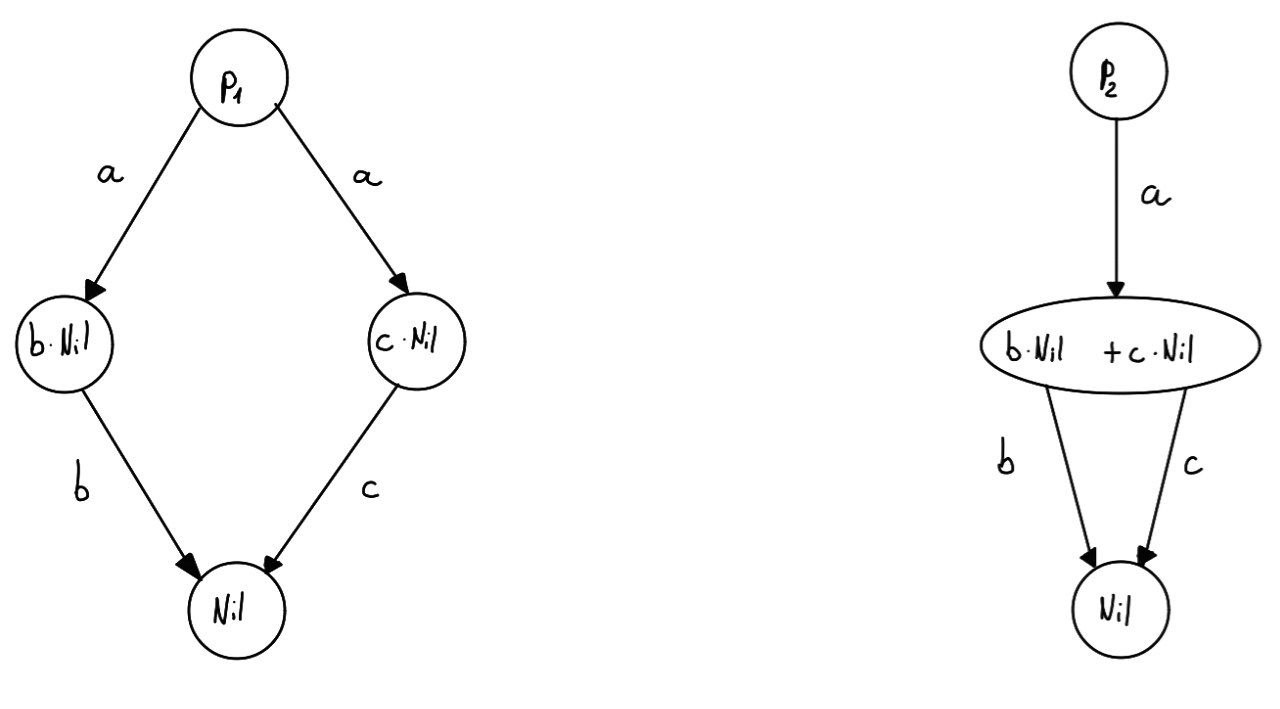
\includegraphics[scale=0.25]{img/ccs/Esempio1.png}
        \caption{LTS dei processi $p_1$ e $p_2$}
    \end{figure}
    Osserviamo subito che i due processi sono equivalenti rispetto alle tracce,
    difatti:
    \begin{itemize}
        \item $Tracce(p_1) = \{\varepsilon, a, a . b, a . c\}$
        \item $Tracce(p_2) = \{\varepsilon, a, a . b, a . c\}$
    \end{itemize}
    Vediamo se i due processi sono anche bisimili.
    \begin{itemize}
        \item Da $p_1$ possiamo eseguire l'azione $a$ e possiamo fare lo stesso
              anche da $p_2$. Dobbiamo però chiederci se gli stati di arrivo sono anche
              essi in relazione di bisimulazione.
        \item Gli stati interessati sono $b . Nil$ e $b . Nil + c . Nil$:
              dal primo possiamo eseguire $b$, che è fattibile anche dal secondo, ma
              dal secondo possiamo eseguire $c$, che non è eseguibile dal primo (la
              bisimulazione richiede che entrambi gli stati siano simili tra loro),
              dunque i due processi non sono bisimili.
    \end{itemize}
    Formalmente:
    \begin{itemize}
        \item $p_1 \xrightarrow{a} b . Nil$
        \item $p_2 \xrightarrow{a} b . Nil + c . Nil$
    \end{itemize}
    $b . Nil \stackrel{Bis}{\not\sim} b . Nil + c . Nil$ inoltre,
    possiamo osservare che: $b . Nil \stackrel{T}{\not\sim} b . Nil + c . Nil$
\end{esempio}
\begin{esempio}
    Consideriamo due processi che simulano dei buffer che possono contenere due
    elementi:
    \begin{itemize}
        \item $B_0^1 | B_0^1$ dove $B_0^1 = in . B_1^1$ e $B_1^1 =
                  \overline{out} . B_0^1$
        \item $B_0^2 = in . B_1^2$, $B_1^2= \overline{out} . B_0^2 + in
                  . B_2^2$ e $B_2^2 = \overline{out} . B_1^2$
    \end{itemize}
    \begin{figure}[!ht]
        \centering
        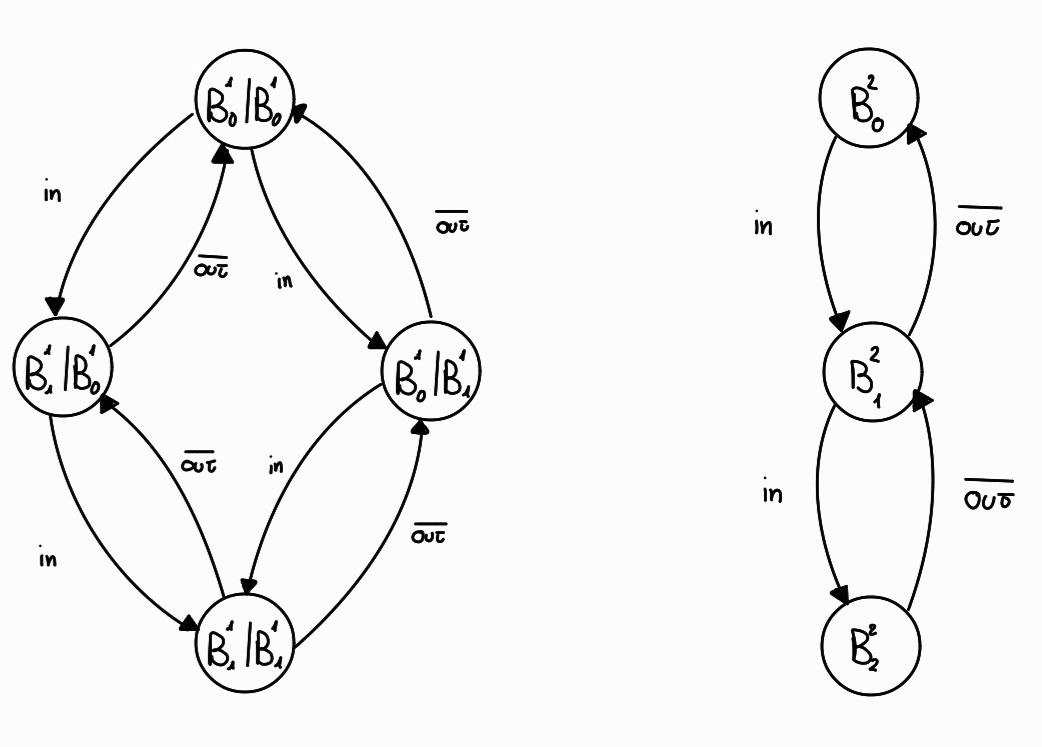
\includegraphics[scale=0.25]{img/ccs/Esempio 2.png}
        \caption{LTS dei processi $B_0^1 | B_0^1$ e $B_0^2$}
    \end{figure}
    In questo esempio, possiamo osservare che: $$(B_0^1 | B_0^1) \stackrel{Bis}{\sim} B_0^2$$
    $B_0^2$ può essere messo in relazione con $B_0^1| B_0^1$ in quanto se vado
    in uno tra $B_1^1 | B_0^1$ e $B_0^1 | B_1^1$ posso sempre fare $in$ e $\overline{out}$.
    Inoltre, Posso fare un discorso analogo per $B_2^2$ e $B_1^1 | B_1^1$.
    Essendo questi ultimi quindi bisimili lo sono anche il nodo centrale coi
    due possibili nodi nel caso della composizione e di conseguenza lo sono
    anche $B_0^2$ e $B_0^1 | B_0^1$.
\end{esempio}
La bisimulazione si può testare mettendo i due processi in parallelo e restringendo
le operazioni, se entrambi arrivano alla fine utilizzando la sincronizzazione
allora sono bisimili.
\begin{osservazione}
    La Bisimulazione forte è una congruenza anche rispetto agli operatori CCS,
    ovvero se $p, q \in Proc_{CCS} \land p \stackrel{Bis}{\sim} q$ allora:
    \begin{itemize}
        \item $\alpha.p \stackrel{Bis}{\sim} \alpha.q$
        \item $p + r \stackrel{Bis}{\sim}q + r$ e $r + p \stackrel{Bis}{\sim} r
                  + q, \forall r \in Proc_{CCS}$
        \item $p | r \stackrel{Bis}{\sim} q | r$ e $r | p \stackrel{Bis}{\sim} r | q
                  \forall r \in Proc_{CCS}$
        \item $\forall f: Act \to Act$ funzione di rietichettatura, se $p[f]
                  \stackrel{Bis}{\sim} q[f]$ allora $p \stackrel{Bis}{\sim} q$
        \item $p_{\setminus L} \stackrel{Bis}{\sim} q_{\setminus L}$ e $L \subseteq
                  Act$
    \end{itemize}
\end{osservazione}
\begin{osservazione}
    Inoltre valgono le seguenti proprietà:
    \begin{itemize}
        \item \textbf{Commutatività rispetto alla somma}: $p + q \stackrel{Bis}{\sim}
                  q + p$
        \item \textbf{Commutatività rispetto alla parallelizzazione}: $p | q
                  \stackrel{Bis}{\sim} q | p$
        \item \textbf{Associatività rispetto alla somma}: $(p + q) + r
                  \stackrel{Bis}{\sim} p + (q + r)$
        \item \textbf{Associatività rispetto alla parallelizzazione}: $(p | q) | r
                  \stackrel{Bis}{\sim} p | (q | r)$
        \item \textbf{Annullamento rispetto alla somma}: $p + Nil \stackrel{Bis}{\sim}
                  p$
        \item \textbf{Annullamento rispetto alla parallelizzazione}: $p | Nil
                  \stackrel{Bis}{\sim} p$
    \end{itemize}
\end{osservazione}
\begin{osservazione}
    Per ogni coppia $p, q \in Proc_{CCS}$ vale:
    \begin{itemize}
        \item $LTS(p)$ isomorfo $LTS(q)$ implica $p \stackrel{Bis}{\sim} q$
        \item Si ha un'astrazione di stati.
        \item $p \stackrel{Bis}{\sim} q \Rightarrow p \stackrel{T}{\sim} q \Rightarrow
                  \stackrel{Bis}{\sim} \subseteq \stackrel{T}{\sim}$
        \item È una congruenza tra gli operatori CCS.
        \item Preserva la stessa probabilità di deadlock (o assenza) nell'interazione
              con l'ambiente.
        \item $\stackrel{Bis}{\sim}$ è troppo restrittiva perché $a.b.Nil
                  \stackrel{Bis}{\not\simeq} a.\tau.b.Nil$. In sostanza $\stackrel{Bis}{\sim}$ e
              $\stackrel{T}{\sim}$ non astraggono le $\tau$.
    \end{itemize}
\end{osservazione}
\subsection{Bisimulazione debole}
La bisimulazione forte rischia di essere troppo restrittiva. Si passa quindi alla
definizione di \textbf{equivalenza debole rispetto alle tracce} $\stackrel{T}{\approx}$
e \textbf{bisimulazione debole} $\stackrel{Bis}{\approx}$.
La definizione di queste nuove relazioni obbliga a modificare la definizione
della funzione di transizione. La relazione di transizione debole è definita come:
\begin{equation}
    \Rightarrow \subseteq Proc_{CCS} \times Act \times Proc_{CCS}
\end{equation}
Possiamo rappresentare tale funzione come $p \stackrel{\alpha}{\Rightarrow} p'$ dove
$\alpha \in Act$ se e solo se:
\begin{itemize}
    \item Se $\alpha = \tau$ allora posso eseguire una sequenza qualsiasi, anche
          nulla, di $\tau$:
          \begin{equation}
              p \xrightarrow{\tau}^{\ast} p'\begin{cases}
                  p = p'
                                        & \text{se non ci sono } \tau \text{ da eseguire} \\
                  p \xrightarrow{\tau} p_1 \xrightarrow{\tau} \dots
                  \xrightarrow{\tau} p' & \text{altrimenti}
              \end{cases}
          \end{equation}
    \item Se $\alpha \in A \cup \overline{A}$ allora vale:
          $p \xrightarrow{\tau}^{\ast} \xrightarrow{\alpha} \xrightarrow{\tau}^{\ast}$
\end{itemize}
Come fatto per la relazione forte, definiamo la relazione di transizione per
sequenze di azioni $w \in Act^{\ast}$ come $p \stackrel{w}{\Rightarrow} p'$ se e solo se:
\begin{itemize}
    \item Se $w = \varepsilon$ oppure $w = \tau^{\ast}$ allora ho:
          \begin{equation}
              p \xrightarrow{\tau}^{\ast} p'
          \end{equation}
    \item Se $w = a_1\dots a_n$ con $a_i \in A \cup \overline{A}$ allora:
          \begin{equation}
              p \stackrel{a_1}{\Rightarrow} p_1 \stackrel{a_2}{\Rightarrow} \dots
              \stackrel{a_n}{\Rightarrow} p'
          \end{equation}
          dove ogni $a_i$ può essere preceduto/seguito da una qualsiasi sequenza
          di $\tau$.
\end{itemize}
\begin{definizione}[\textbf{Equivalenza debole rispetto alle tracce}]
    Definiamo l'\textbf{equivalenza debole rispetto alle tracce}, la quale è
    rappresentata come $p \stackrel{T}{\approx} q$ se e solo se:
    \begin{equation}
        tracce_{\Rightarrow} (p) = tracce_{\Rightarrow}(q) \ \text{ovvero} \
        \forall w \in (A \cup \overline{A}) \ \text{ho che} \ p
        \stackrel{w}{\Rightarrow} \iff q \stackrel{w}{\Rightarrow}
    \end{equation}
    quindi se i due processi possono eseguire la stessa sequenza di azioni.
\end{definizione}
Posso definire le tracce come:
\begin{equation}
    tracce_{\Rightarrow}(p) = \{w \in (A \cup \overline{A})^{\ast} | p
    \stackrel{w}{\Rightarrow}\}
\end{equation}
\begin{osservazione}
    In primis si ha che:
    \begin{equation}
        p \stackrel{T}{\sim} q \Rightarrow p \stackrel{T}{\approx} q \Rightarrow
        \stackrel{T}{\sim} \subseteq \stackrel{T}{\approx}
    \end{equation}
    Per ogni coppia $p, q \in Proc_{CCS}$ vale:
    \begin{itemize}
        \item $LTS(p)$ isomorfo $LTS(q)$ implica $p \stackrel{T}{\approx} q$
        \item Si ha un'astrazione di stati.
        \item È una congruenza tra gli operatori CCS.
        \item Non preserva la stessa probabilità di deadlock (o assenza)
              nell'interazione con l'ambiente.
    \end{itemize}
\end{osservazione}
\begin{definizione}[\textbf{Bisimulazione debole}]
    Data una relazione $R$ definita come $R \subseteq Proc_{CCS} \times Proc_{CCS}$.
    Dico che $R$ è una relazione di \textbf{bisimulazione debole} se e solo se:
    \begin{equation}
        \forall p, q \in Proc_{CCS} \ \text{tale che } p R q \ \text{vale che }
        \forall a \in Act
    \end{equation}
    \begin{itemize}
        \item Se $p \xrightarrow{a} p'$ allora $\exists q'$ tale che
              $q \stackrel{a}{\Rightarrow} q'$ e $p'Rq'$
        \item E deve valere anche il viceversa: $q \xrightarrow{a} q'$ allora
              $\exists p'$ tale che $p \stackrel{a}{\Rightarrow} p'$ e $p'Rq'$
    \end{itemize}
\end{definizione}
Due processi $p$ e $q$ sono in relazione di bisimulazione debole $p
    \stackrel{Bis}{\approx} q$
se e solo se esiste una relazione di bisimulazione $R$ tale che $p R q$ si ha che vale:
\begin{equation}
    \stackrel{Bis}{\approx} = \bigcup \{R | R \ \text{è di bisimulazione debole}\}
\end{equation}
\begin{esempio}
    Consideriamo i processi $r = a . (b . Nil + \tau . c . Nil)$
    e $k = a . (b . Nil + \tau . c . Nil) + a . c . Nil$.
    \begin{figure}[!ht]
        \centering
        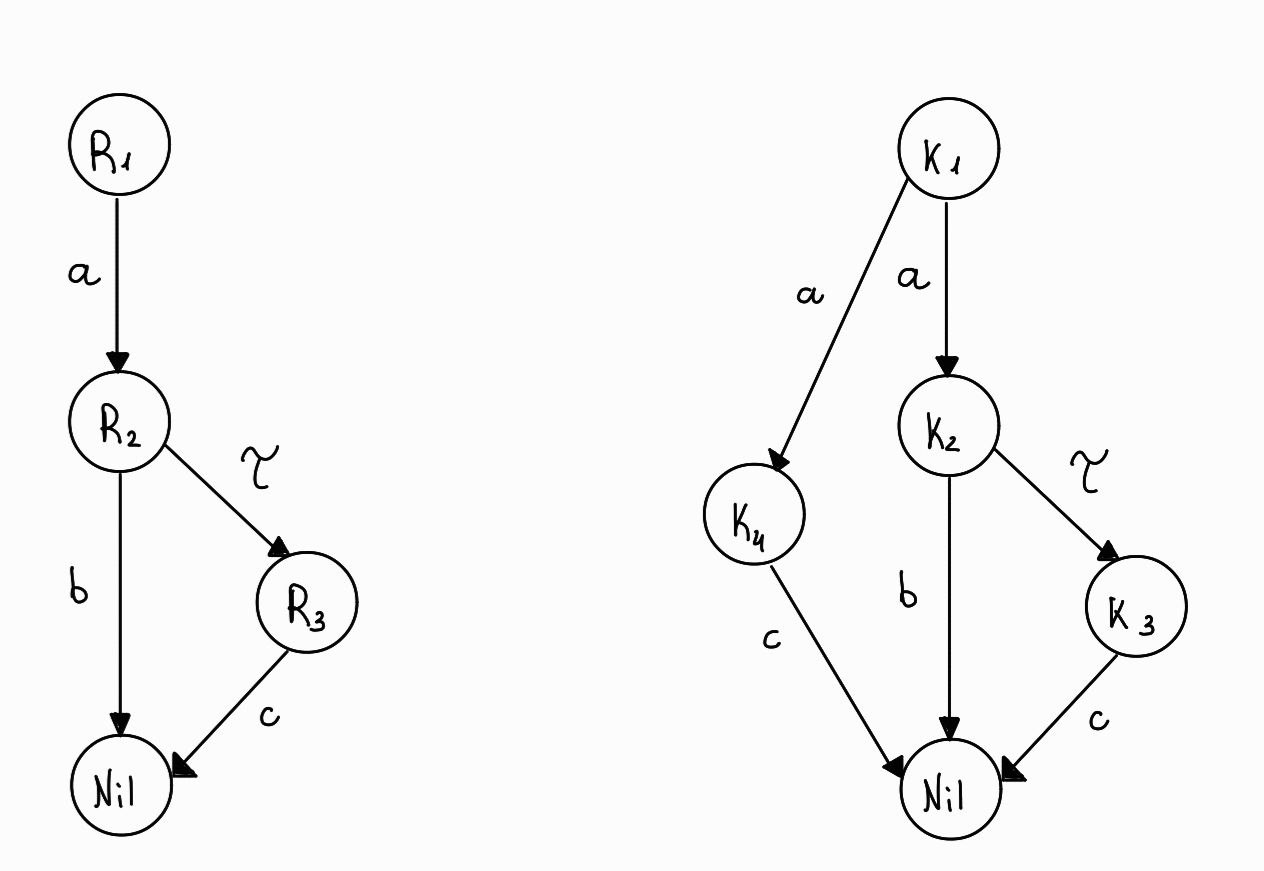
\includegraphics[scale=0.25]{img/ccs/Esempio3.png}
        \caption{LTS di $r$ e $k$}
    \end{figure}
    $$r \stackrel{Bis}{\approx} k$$
\end{esempio}
\begin{definizione}[\textbf{Processo deterministico}]
    Sia $p \in Proc_{CCS}$ è un processo deterministico se e solo se vale che:
    \begin{equation}
        \forall \alpha \in Act, \ p \xrightarrow{\alpha} p' \land p
        \xrightarrow{\alpha} p'' \Rightarrow p' = p''
    \end{equation}
\end{definizione}
\begin{osservazione}
    Siano $p, q \in Proc_{CCS}$, se $p, q$ sono deterministici e $p \stackrel{T}{\sim}
        q$ ($p \stackrel{T}{\approx} q$) allora $p \stackrel{Bis}{\sim}
        q$ ($p \stackrel{Bis}{\approx} q$).
\end{osservazione}
\begin{osservazione}
    Le proprietà della relazione di bisimulazione debole sono:
    \begin{itemize}
        \item È un'equivalenza.
        \item Preserva la possibilità di generare (o non generare) deadlock
              nell'interazione con l'ambiente (non ci sono problemi con i deadlock).
        \item Astraiamo dagli stati, azioni inosservabili ($\tau$) e dai cicli.
              \begin{equation}
                  Nil \stackrel{Bis}{\approx} \tau . p
              \end{equation}
    \end{itemize}
\end{osservazione}
La bisimulazione debole \textbf{non} è una congruenza rispetto agli operatori CCS.
\begin{teorema}
    Se $p, q \in Proc_{CCS}$, $p \stackrel{Bis}{\approx} q$ allora:
    \begin{itemize}
        \item $\alpha . p \stackrel{Bis}{\approx} \alpha . q, \forall \alpha \in A$
        \item $p | r \stackrel{Bis}{\approx} q | r \land r | p \stackrel{Bis}{\approx}
                  r | q, \forall r \in Proc_{CCS}$
        \item $p[f] \stackrel{Bis}{\approx} q[f], \forall f: Act \to Act$ funzione
              di rietichettatura.
        \item $p_{\setminus L} \stackrel{Bis}{\approx} q_{\setminus L}, \forall
                  L \subseteq Act$
        \item Rispetto all'operatore $+$ e alla ricorsione questa cosa non è vera:
              \begin{equation}
                  \tau . a . Nil \stackrel{Bis}{\approx} a.Nil, \tau . a . Nil + b.Nil
                  \stackrel{Bis}{\not\approx} a.Nil + b.Nil
              \end{equation}
    \end{itemize}
\end{teorema}
\subsubsection{Congruenza}
Possiamo cercare la più grande relazione di congruenza $\stackrel{C}{\approx}$
che più si avvicina a $\stackrel{Bis}{\approx}$.
\begin{equation}
    \stackrel{C}{\approx} \subseteq \stackrel{Bis}{\approx} \subseteq Proc_{CCS}
    \times Proc_{CCS}
\end{equation}
Non sarà altro che una bisimulazione ristretta senza ricorsione e con processi
(agenti) finiti. Per fare ciò dovremo definire un insieme finito di assiomi $Ax$
che permetta di dimostrare la congruenza, tale che:
\begin{itemize}
    \item Ax \textit{corretto} ($Ax \vdash p = q \Rightarrow p \stackrel{C}{\approx} q$)
    \item Ax \textit{completo} ($p \stackrel{C}{\approx} q \Rightarrow Ax \vdash p = q$)
\end{itemize}
\begin{enumerate}
    \item \textbf{Legge associativa}:
          \begin{equation}
              p + (q + r) \stackrel{C}{\approx} (p + q) + r \ \text{e} \ p | (q | r)
              \stackrel{C}{\approx} (p | q) | r
          \end{equation}
    \item \textbf{Legge commutativa}:
          \begin{equation}
              p + q \stackrel{C}{\approx} q + p \ \text{e} \ p | q
              \stackrel{C}{\approx} q | p
          \end{equation}
    \item \textbf{Legge di assorbimento}:
          \begin{equation}
              p + p \stackrel{C}{\approx} p \ (\text{ma} \ p | p
              \stackrel{C}{\not\approx} p)
          \end{equation}
    \item $p + Nil \stackrel{C}{\approx} p$ e $p | Nil \stackrel{C}{\approx} p$
    \item $p + \tau . p \stackrel{C}{\approx} \tau . p$
    \item $\mu . \tau . p \stackrel{C}{\approx} \mu . p$
    \item $\mu . (p + \tau . q) \stackrel{C}{\approx} \mu . (p +
              \tau . q) + \mu . q$
    \item Se $p$ e $q$ sono delle somme: $p = \sum_{i} \alpha_i . p_i$ e
          $q = \sum_{j} \beta_j . q_j$,  $\alpha, \beta \in Act$:
          $$p | q \stackrel{C}{\approx} \sum_{i} \alpha_i (p_{i} | q) + \sum_{j}
              \beta_{j} . (p|q_{j}) + \sum_{\alpha_i = \overline{\beta}_{j}}
              \tau . (p_{i} | q_{j})$$
          (\textbf{Teorema di espansione di R. Milner}) Questo assioma mi permette
          di rappresentare la composizione parallela come la somma di tutte le
          possibili alternative che si hanno con l'operazione di composizione
          parallela.
    \item $p[f] \stackrel{C}{\approx} \sum_{i} f(\alpha_i) . (p_{i} [f])$ $\forall f$
          funzione di etichettatura.
    \item $p_{\backslash L} \stackrel{C}{\approx} \sum_{\alpha_i,\overline{\alpha}_i
                  \not\in L} \alpha_i . (pi_{\backslash L})$ $\forall L \subseteq A$
\end{enumerate}
Il problema della bisimulazione è che confronta i processi in base alle azioni che
devono essere atomiche, se dovessimo raffinare un'azione in 2 più piccole allora
le equivalenze di bisibulazione perdono effetto.

Dal momento che gli LTS hanno un esecuzione non deterministica e questo
non permette di evidenziare le dipendenze o le indipendenze, per questo sono
state create le reti di petri.
\subsubsection{Gioco verifica bisimulazione debole}
Per confrontare due processi $p$ e $q$ si può utilizzare un gioco $G(p, q)$ con
2 giocatori:
\begin{itemize}
    \item \textbf{Attaccante}: il quale cerca di dimostrare che $p
              \stackrel{Bis}{\not\approx} q$
    \item \textbf{Difensore}: il quale cerca di dimostrare che $p
              \stackrel{Bis}{\approx} q$
\end{itemize}
Un gioco è composto da più partite, dove ogni partita è una sequenza finita o
infinita di configurazioni: $$(p_0, q_0), (p_1, q_1), \dots, (p_i, q_i), \dots$$
In ogni mano si passa dalla configurazione corrente $(p_i, q_i)$ alla successiva
$(p_{i + 1}, q_{i + 1})$ con le seguenti regole:
\begin{itemize}
    \item L'Attaccante sceglie uno dei due processi della configurazione corrente
          $(p_i, q_i)$ e fa una $\xrightarrow{\alpha}$ mossa $(\alpha \in Act)$
    \item Il Difensore deve rispondere con una $\stackrel{\alpha}{\Rightarrow}$
          mossa nell'altro processo.
\end{itemize}
La coppia di processi $(p_{i+1}, q_{i+1})$ così ottenuta diventa la nuova
configurazione corrente. La partita continua con un'altra mano.

La partita può terminare in uno dei due seguenti modi:
\begin{itemize}
    \item Se un giocatore non può muovere, l'altro vince.
    \item Se la partita è infinita, vince il difensore.
\end{itemize}
Diverse partite possono concludersi con vincitori diversi, ma per ogni gioco, un
solo giocatore può vincere ogni partita.

Una \textbf{strategia} per un giocatore è un insieme di regole che indicano di
volta in volta che mossa fare. Tali regole dipendono solo dalla configurazione
corrente. Un giocatore ha una \textbf{strategia vincente} per un gioco $G(p, q)$
se seguendo quella strategia è in grado di vincere tutte le partite del gioco.
\begin{teorema}
    Per ogni gioco $G(p, q)$, solo uno dei due giocatori ha una strategia vincente.
    \begin{itemize}
        \item L'Attaccante ha una strategia vincente per $G(p, q)$ se e solo se
              $p \stackrel{Bis}{\not\approx} q$.
        \item Il Difensore ha una strategia vincente per $G(p, q)$ se e solo se
              $p \stackrel{Bis}{\approx} q$.
    \end{itemize}
\end{teorema}
\begin{nota}
    Il gioco della bisimulazione può essere usato sia per dimostrare che due
    processi sono bisimili, che per dimostrare che non lo sono.
\end{nota}
Per dimostrare che i processi sono bisimili, bisogna mostrare che il Difensore
ha una strategia vincente, cioè che, per ogni mossa dell'Attaccante, il Difensore
ha almeno una mossa che lo porterà a vincere.

Per dimostrare che i processi \textbf{non} sono bisimili, bisogna mostrare che
l'Attaccante ha una strategia vincente, cioè che, in ogni configurazione,
l'Attaccante è in grado di scegliere su quale processo operare e con quale azione,
in modo che per ogni successiva mossa del Difensore, l'Attaccante ha almeno una
mossa che lo porterà a vincere.
\chapter{Reti di Petri}
Abbiamo introdotto un'algebra di processi come CCS dove processi sequenziali
interagiscono tra loro tramite hand-shaking. Un altro modello usato, con varie
implementazioni, sono gli automi a stati finiti. Si passa ora alle reti di Petri.

La critica di Petri è che in un sistema distribuito non sia individuabile uno
stato globale, che in un sistema distribuito le trasformazioni di stato siano
localizzate e non globali, che non esista un sistema di riferimento temporale
unico. Quindi la simulazione sequenziale non deterministica (semantica a
“interleaving”) dei sistemi distribuiti è una forzatura e non rappresenta le
reali caratteristiche del comportamento del sistema, ovvero la località, la
distribuzione degli eventi e la relazione di dipendenza causale e non causale
tra gli eventi.

Nel modello proposto da Petri, le azioni vengono rappresentate come nodi
dell'automa e non più come etichette della transizione. Oltre a ciò, le azioni e
le coazioni che abbiamo definito in CCS per sincronizzare due processi diventano
una singola azione di sincronizzazione.

Petri sviluppò una teoria matematica fondata sui principi della fisica moderna,
che sia una teoria dei sistemi in grado di descrivere il flusso di informazione
e permetta di analizzare sistemi con organizzazione complessa.

Lo \textbf{stato} è definito da una collezione di stati locali.
\section{Reti elementari}
\begin{definizione}[\textbf{Rete}]
    Una \textbf{rete} è definite come:
    \begin{equation}
        N = (B, E, F)
    \end{equation}
    dove:
    \begin{itemize}
        \item $B$ è un insieme finito di condizioni, anche detti stati locali,
              proposizioni vere o false. Rappresentato da: $$\bigcirc$$
        \item $E$ è un insieme finito di eventi, \textbf{trasformazioni locali}
              di stato. Rappresentato da: $$\Box$$
              \begin{equation}
                  B\cap E  = \emptyset \land B\cup E \ne \emptyset
              \end{equation}
        \item $F \subseteq (B \times E) \cup (E \times B)$ è una
              \textbf{relazione di flusso} Rappresentato da: $$\to$$
              Inoltre, la relazione di flusso è tale per cui non esistano elementi
              isolati, in quanto non avrebbero senso. Si ha, formalmente, che:
              \begin{equation}
                  dom(F) \cup ran(F) = B \cup E
              \end{equation}
              ovvero non ho condizioni/eventi isolati, in quanto non avrebbero
              senso, avrei una condizione costante e un evento che non accade
              mai; quindi, dominio e codominio di $F$ coprono l'insieme di
              condizioni ed eventi.
    \end{itemize}
\end{definizione}
Sia $x \in X$ dove l'insieme $X$ è definito come $X = B \cup E$, allora possiamo
definire:
\begin{itemize}
    \item $^{\bullet} x =\{y \in X: \ (y, x) \in F\}$ sono i \textbf{pre-elementi}
          di $x$. Posso anche definirli come precondizioni o pre-eventi.
    \item $x^{\bullet} =\{y \in X: \ (x, y) \in F\}$ sono i \textbf{post-elementi}
          di $x$. Posso anche definirli come post-condizioni o post eventi.
\end{itemize}
Sia $A \subseteq B \cup E$ allora posso definire:
\begin{itemize}
    \item $^{\bullet} A = \bigcup_{x \in A} \ ^{\bullet} x$
    \item $A^{\bullet} = \bigcup_{x \in A} x^{\bullet}$
\end{itemize}
Nelle reti c'è sempre una relazione di dualità tra due elementi, per esempio tra
condizioni ed eventi, tra pre-eventi e post-eventi, tra precondizioni e post
condizioni. Inoltre, si ha la caratteristica della località, quindi si hanno stati
locali e trasformazioni di stato locali.

La rete $N = (B, E, F)$ descrive la struttura statica del sistema, il
comportamento è definito attraverso le nozioni di caso e di regola di scatto o
regola di transizione.

Un \textbf{caso} o \textbf{configurazione} è un insieme di condizioni $c \subseteq B$
che rappresentano l'insieme di condizioni vere in una certa configurazione del
sistema, un insieme di stati locali che collettivamente individuano lo
\textit{stato globale} del sistema.
\begin{itemize}
    \item Condizione vera: $$\bigodot$$
    \item Condizione falsa: $$\bigcirc$$
\end{itemize}
\begin{definizione} [\textbf{Regola dello scatto}]
    Sia $N = (B, E, F)$ una rete elementare e $c \subseteq B$. L'evento $e \in E$
    è \textbf{abilitato}, ovvero può occorrere, in $c$, denotato $c[e >$, se e
    solo se:
    \begin{equation}
        ^{\bullet} e \subseteq c \ \land \ e^{\bullet} \cap c = \emptyset
    \end{equation}
    Se $c[e >$, allora quando $e$ occorrere in $c$ genera un nuovo caso $c'$,
    denotato $c[e > c'$:
    \begin{equation}
        c' = (c - ^{\bullet} e) \cup e^{\bullet}
    \end{equation}
\end{definizione}
In altre parole, un evento $e$ è abilitato se le sue precondizioni sono vere,
le post-condizioni false. Lo scatto di $e$ rende le precondizioni false e le
post-condizioni vere, le altre condizioni rimangono inalterate.

Le reti si basano sul \textbf{principio di estensionalità}, ovvero sul fatto che
il cambiamento di stato è locale:
\begin{center}
    \textit{Un evento è completamente caratterizzato dai cambiamenti che produce
        negli stati locali, tali cambiamenti sono indipendenti dalla particolare
        configurazione in cui l'evento occorre.}
\end{center}
\begin{definizione}[]
    Sia $N = (B, E, F)$ una \textbf{rete elementare}, si ha che:
    \begin{itemize}
        \item $N$ è \textbf{semplice} se e solo se:
              \begin{equation}
                  \forall x, y \in B \cup E, \ ^{\bullet} x = \ ^{\bullet} y \
                  \land \ x^{\bullet} = y^{\bullet} \Rightarrow x = y
              \end{equation}
        \item $N$ è \textbf{pura} se e solo se:
              \begin{equation}
                  \forall e \in E: \ ^{\bullet}e \cap e^{\bullet} = \emptyset
              \end{equation}
    \end{itemize}
\end{definizione}
\begin{definizione}
    Sia $N = (B, E, F)$ una rete elementare, $U \subseteq E$ e $c, c_1, c_2 \subseteq B$.
    \begin{itemize}
        \item $U$ è un \textbf{insieme di eventi indipendenti} se e solo se:
              \begin{equation}
                  \forall e_1, e_2 \in U: \ e_1 \neq e_2 \Rightarrow (^{\bullet}e_1
                  \cup e_1^{\bullet}) \cap (^{\bullet}e_2 \cup e_2^{\bullet}) = \emptyset
              \end{equation}
        \item $U$ è un \textbf{passo abilitato} (insieme di eventi concorrenti)
              in $c$ anche scritto come $c[U >$ se e solo se:
              \begin{equation}
                  U \ \text{insieme di eventi indipendenti} \ \land \ \forall e
                  \in U: \ c[e >
              \end{equation}
        \item $U$ è un \textbf{passo} da $c_1$ a $c_2$, anche scritto come
              $c_1[U > c_2$ se e solo se:
              \begin{equation}
                  c_1 [ U > \ \land \ c_2 = (c_1 - \ ^{\bullet} U) \cup U^{\bullet}
              \end{equation}
    \end{itemize}
    Se due eventi sono indipendenti allora pososno eseguire concorrentemente.
\end{definizione}
Un \textbf{sistema elementare} $\Sigma = (B, E, F; c_{in})$ è definito da una rete
$N = (B, E, F)$ e da $c_{in} \subseteq B$ un caso iniziale.
\begin{definizione}[\textbf{Caso raggiungibile}]
    L'insieme dei \textbf{casi raggiungibili} ($C_{\Sigma}$) del sistema elementare
    $\Sigma = (B, E, F; c_{in})$ è il più piccolo sottoinsieme di $2^B$ tale che:
    \begin{itemize}
        \item $c_{in} \in C_{\Sigma}$
        \item Se $c \in C_{\Sigma}, U \subseteq E, c' \subseteq B$ sono tali che:
              $c[U > c'$ allora $c' \in C_{\Sigma}$
    \end{itemize}
\end{definizione}
L'insieme $C_\Sigma$ è un insieme \textbf{finito} perché si parla di sottoinsiemi
di insiemi finiti che sono anch'essi finiti, ovviamente esplode in un esponenziale.
\begin{definizione}[\textbf{Insieme dei passi}]
    $U_{\Sigma}$ è l'\textbf{insieme dei passi} di $\Sigma$:
    \begin{equation}
        U_{\Sigma} = \{U \subseteq \ E | \exists c, c' \in C_{\Sigma}: c[U > c'\}
    \end{equation}
\end{definizione}
Sia $\Sigma = (B, E, F; c_{in})$ un sistema elementare,
$c_i \in C_{\Sigma}, e_i \in E, U_i \subseteq E$ possiamo distinguere:
\begin{itemize}
    \item \textbf{Comportamento sequenziale}: sequenze di occorrenze o di eventi
          (”interleaving”, simulazione sequenziale non deterministica), ovvero una
          sequenza di eventi che possono occorrere dal caso iniziale, facendo scattare
          in maniera sequenziale gli eventi uno alla volta in $c_n$:
          \begin{equation}
              c_{in}[e_1 > c_1[e_2 > \dots [e_n > c_n \ \text{oppure} \
              c_{in}[e_1e_2 \dots e_n > c_n
          \end{equation}
    \item \textbf{Comportamento non sequenziale} (semantica a passi): sequenze di
          passi (”step semantics”) in quanto possiamo anche considerare insiemi
          di eventi, ovvero passi:
          \begin{equation}
              c_{in}[U_1 > c_1[U_2 > \dots [U_n > c_n \ \text{oppure} \
              c_{in}[U_1U_2 \dots U_n > c_n
          \end{equation}
    \item \textbf{Comportamento non sequenziale}  (semantica di ordine parziale):
          processi non sequenziali (”partial order semantics” - ”true concurrency”).
          Il comportamento di tale sistema viene registrato in una rete di Petri.
\end{itemize}
Si considerano sia sequenze finite che sequenze infinite (di eventi o di passi).

Il comportamento di un sistema elementare $\Sigma = (B, E, F; c_{in})$ può essere
rappresentato dal suo grafo dei casi.
\begin{definizione}[\textbf{Grafo dei casi}]
    Il \textbf{grafo dei casi} di $\Sigma$ è il sistema di transizioni etichettato
    $CG_{\Sigma} = (C_{\Sigma},U_{\Sigma}, A, c_{in})$ dove:
    \begin{itemize}
        \item $C_{\Sigma}$ è l'insieme dei nodi del grafo (gli stati globali).
        \item $U_{\Sigma}$ è l'alfabeto.
        \item $A$ è l'insieme di archi etichettati:
              \begin{equation}
                  A = \{(c, U, c') | c, c' \in C_{\Sigma}, U \in U_{\Sigma}, c[U > c'\}
              \end{equation}
              I nodi sono i casi sequenziali mentre gli archi sono gli insiemi
              di eventi indipendenti
    \end{itemize}
\end{definizione}
\begin{definizione}[\textbf{Grafo dei casi sequenziale}]
    Il \textbf{grafo dei casi sequenziali} di $\Sigma=(B,E,F;c_{in})$ è
    il sistema di transizioni etichettato $SCG_\Sigma=(C_\Sigma, E, A,c_{in})$
    dove:
    \begin{equation}
        A=\left\{(c,e,c')|c,c'\in C_\Sigma, e\in E: c[e>c' \right\}
    \end{equation}
    I nodi sono i casi sequenziali mentre gli archi sono gli eventi
\end{definizione}

\subsection{Diamond property}
\begin{definizione} [\textbf{Diamond property}]
    Sia $\Sigma = (B, E, F; c_{in})$ un sistema elementare,
    $CG_{\Sigma} = (C_{\Sigma},U_{\Sigma}, A, c_{in})$ il suo grafi dei casi,
    $U_1,U_2 \in U_{\Sigma}: U_1 \cap U_2 = \emptyset, U_1 \neq \emptyset, U_2
        \neq \emptyset$, e $c_1, c_2, c_3, c_4 \in C_{\Sigma}$, allora valgono:
    \begin{enumerate}
        \item Dato $c_1[e_1 >$ e $c_1[e_2 >$ segue che:
              \begin{equation}
                  ^{\bullet}e_1 \cap e_2^{\bullet} = \emptyset \ \land \
                  ^{\bullet}e_2 \cap e_1^{\bullet} = \emptyset
              \end{equation}
              infatti, se $e_1$ e $e_2$ sono entrambi abilitati in $c_1$, le loro
              precondizioni sono vere e le post-condizioni false, e quindi non è
              possibile che una condizione sia contemporaneamente precondizione di
              $e_1$ (vera) e anche post-condizione di $e_2$ (falsa), e viceversa.

              Da $c_1[e_1 > c_2[e_2  >$ segue:
              \begin{equation}
                  ^{\bullet} e_1 \cap ^{\bullet} e_2 = \emptyset \ \land \
                  e_1^{\bullet} \cap e_2^{\bullet} = \emptyset
              \end{equation}
              in $c_2$, infatti, le precondizioni di $e_1$ sono false mentre le
              precondizioni di $e_2$ sono vere e quindi $e_1$ e $e_2$ non possono
              avere precondizioni in comune. Inoltre, sempre in $c_2$ le post-condizioni
              di $e_1$ sono vere, mentre quelle di $e_2$ sono false, e quindi
              $e_1$ e $e_2$ non possono avere post-condizioni in comune. Segue
              quindi \ref{fig:dp1}.
              \begin{figure}[!ht]
                  \centering
                  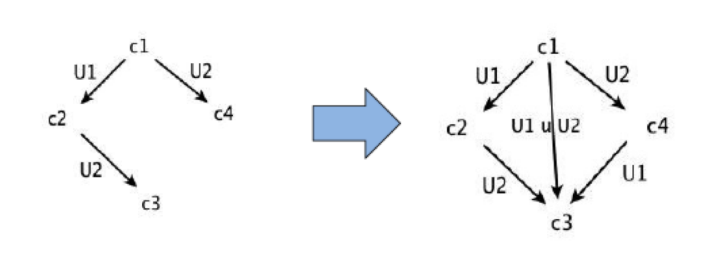
\includegraphics[width=0.5\textwidth]{img/reti/dp1.png}
                  \caption{Diamond property 1}
                  \label{fig:dp1}
              \end{figure}
        \item Supponiamo che $U_1 \cup U_2 \in U_{\Sigma}$ e che
              $U_1 \cap U_2 = \emptyset$, $U_1 \neq \emptyset, U_2 \neq \emptyset$.
              Allora se $c_1[U_1 \cup U_2 >c_3$ sicuramente $c_1[U_1 >$ e $c_1[U_2 >$
              e anche: $c_1[U_1 > c_2[U_2 >c_3$ e $c_1[U_2 > c_4[U_1 >c_3$. Segue
              quindi \ref{fig:dp2}.
              \begin{figure}[!ht]
                  \centering
                  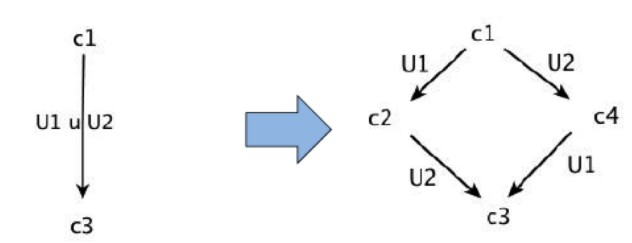
\includegraphics[width=0.5\textwidth]{img/reti/dp2.png}
                  \caption{Diamond property 2}
                  \label{fig:dp2}
              \end{figure}
    \end{enumerate}
\end{definizione}
Per la \textit{Diamond property}, nei sistemi elementari il grafo dei casi e il
grafo dei casi sequenziale sono \textit{sintatticamente equivalenti}, ovvero
possono essere ricavati l'uno dall'altro.

Questo implica il fatto che due sistemi elementari hanno grafi dei casi isomorfi
se e solo se hanno grafi dei casi sequenziale isomorfi.
\begin{definizione}[\textbf{Equivalenza tra sistemi}]
    Due sistemi $\Sigma_1$ e $\Sigma_2$ sono \textbf{equivalenti} se e solo se
    hanno grafi dei casi sequenziali, e quindi anche grafi dei casi, \textbf{isomorfi}.
\end{definizione}
\begin{definizione}[\textit{Problema della sintesi}]
    Dato un sistema di transizioni etichettato $A = (S, E,T,s_0)$, stabilire se
    esiste un sistema elementare $\Sigma = (B, E, F; c_{in})$ tale che: il suo
    grafo dei casi $SCG_{\Sigma}$ sia isomorfo ad $A$. E, in caso affermativo,
    costruire $\Sigma$.

    Questo problema è stato risolto usando la teoria delle regioni. Oltre a ciò,
    A dovrà soddisfare la Diamond property.
\end{definizione}
\begin{definizione}[\textbf{Contatto}]
    Sia $\Sigma = (B, E, F; c_{in})$ un sistema elementare, $e \in E$, $c \in
        C_{\Sigma}$ allora $(e, c)$ è un \textbf{contatto} se e solo se:
    \begin{equation}
        ^{\bullet}e \subseteq c \ \land \ e^{\bullet} \cap c \neq \emptyset
    \end{equation}
\end{definizione}
\begin{definizione}[\textbf{Sistema senza contatti}]
    Un sistema elementare $\Sigma = (B, E, F; c_{in})$ è \textbf{senza contatti}
    se e solo se:
    \begin{equation}
        \forall e \in E, \ \forall c \in C_{\Sigma} \ \text{si ha} \ ^{\bullet}e
        \subseteq c \Rightarrow e^{\bullet} \cap c = \emptyset
    \end{equation}
\end{definizione}
È possibile trasformare un sistema elementare $\Sigma$ con contatti in un
sistema elementare $\Sigma_0$ che sia senza contatti aggiungendo a $\Sigma$ il
complemento di ogni condizione si ottiene un sistema $\Sigma_0$ con grafo dei
casi isomorfo a quello di $\Sigma$.
\begin{figure}[!ht]
    \centering
    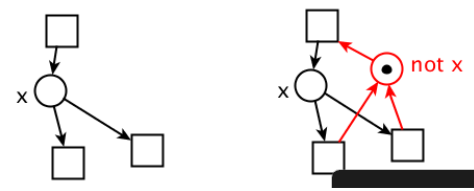
\includegraphics[width=0.5\textwidth]{img/reti/DelContatti.png}
    \caption{Complemento dell'operazione x.}
\end{figure}
Quindi se un sistema elementare $\Sigma$ è senza contatti allora per verificare
che un evento $e$ sia abilitato in un caso raggiungibile $c$ è sufficiente
verificare che le precondizioni di $e$ siano vere:
\begin{equation}
    c[e> \ \text{se e solo se} \ ^{\bullet} e \subseteq c
\end{equation}
\begin{definizione}[\textbf{Sequenza}]
    Sia $\Sigma = (B, E, F; c_{in})$ un sistema elementare, $c \in C_{\Sigma}$
    $e_1, e_2, \in E$, allora $e_1$ ed $e_2$ sono in \textbf{sequenza} in $c$
    se e solo se:
    \begin{equation}
        c[e_1 > \ \land \ \lnot c[e_2 > \ \land \ c[e_1e_2 > \ (c[e_1 > c'[e_2 >)
    \end{equation}
    \begin{figure}[!ht]
        \centering
        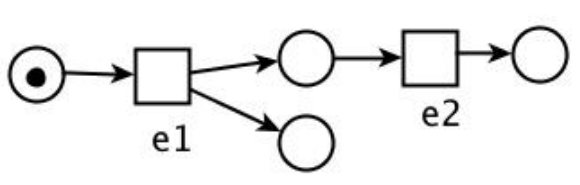
\includegraphics[width=0.5\textwidth]{img/reti/Seq.png}
        \caption{Rappresentazione della sequenza}
    \end{figure}
    In altre parole, è presente una relazione di dipendenza causale tra $e_1$ ed
    $e_2$.
\end{definizione}
\begin{definizione}[\textbf{Concorrenti}]
    Sia $\Sigma = (B, E, F; c_{in})$ un sistema elementare, $c \in C_{\Sigma}$
    $e_1, e_2, \in E$, allora $e_1$ ed $e_2$ sono \textbf{concorrenti} in $c$
    se e solo se:
    \begin{equation}
        c[\{e_1, e_2\} >
    \end{equation}
    \begin{figure}[!ht]
        \centering
        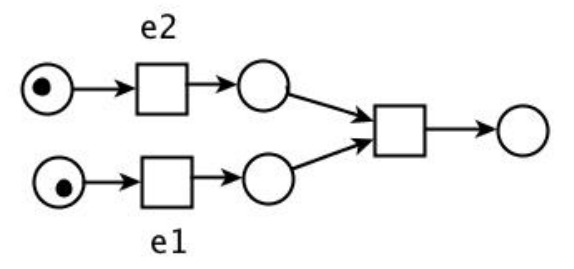
\includegraphics[width=0.5\textwidth]{img/reti/conc.png}
        \caption{Rappresentazione della concorrenza}
    \end{figure}
    In altre parole, se e sol se $e_1$ ed $e_2$ sono indipendenti ed entrambi
    abilitati in $c$.
\end{definizione}
\begin{definizione}[\textbf{Conflitto}]
    Sia $\Sigma = (B, E, F; c_{in})$ un sistema elementare,
    $c \in C_{\Sigma}$ $e_1, e_2, \in E$, allora $e_1$ ed $e_2$ sono in
    \textbf{conflitto} in $c$ se e solo se:
    \begin{equation}
        c[e_1 > \ \land \ c[e_2 > \ \land \ \lnot c[\{e_1, e_2\} >
    \end{equation}
    \begin{figure}[!ht]
        \centering
        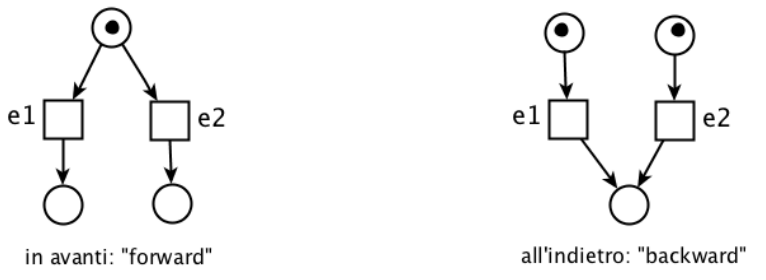
\includegraphics[width=0.5\textwidth]{img/reti/conf.png}
        \caption{Rappresentazione di un conflitto}
    \end{figure}
    In altre parole, sono entrambi abilitati ma l'occorrenza di uno disabilita
    l'altro.
\end{definizione}
Si definisce \textbf{confusione} quando non è possibile stabilire se è stato
risolto un conflitto.
\begin{definizione}[\textbf{Sottorete}]
    Siano $N = (B, E, F)$ e $N_1 = (B_1, E_1, F_1)$ due reti elementari. Diciamo che:
    \begin{itemize}
        \item $N_1 = (B_1, E_1, F_1)$ è \textbf{sottorete} di $N$ se e solo se:
              \begin{itemize}
                  \item $B_1 \subseteq B$
                  \item $E_1 \subseteq E$
                  \item $F_1 = F \cap [(B_1 \times E_1) \cup (E_1 \times B_1)]$
              \end{itemize}
        \item $N_1 = (B_1, E_1, F_1)$ è \textbf{sottorete generata da} $B_1$ se e solo se:
              \begin{itemize}
                  \item $B_1 \subseteq B$
                  \item $E_1 \subseteq ^{\bullet} B_1 \cup B_1^{\bullet}$
                  \item $F_1 = F \cap [(B_1 \times E_1) \cup (E_1 \times B_1)]$
              \end{itemize}
        \item $N_1 = (B_1, E_1, F_1)$ è \textbf{sottorete generata da} $E_1$ se e solo se:
              \begin{itemize}
                  \item $B_1 \subseteq ^{\bullet} E_1 \cup E_1^{\bullet}$
                  \item $E_1 \subseteq E$
                  \item $F_1 = F \cap [(B_1 \times E_1) \cup (E_1 \times B_1)]$
              \end{itemize}
    \end{itemize}
\end{definizione}
Data una rete $N = (B,E, F, c_0)$ questa può essere ottenuta componendo altre
reti di Petri. Si hanno in letteratura 3 modi principali:
\begin{enumerate}
    \item La composizione sincrona: si sincronizzano le retti con un'azione
    \item La composizione asincrona: si sincronizzano le reti con uno stato
    \item La composizione mista tra sincrona e asincrona.
\end{enumerate}
\section{Processi non sequenziali}
Prendiamo l'esempio di una rete ciclica per spegnere il fuoco (fig \ref{fig:spegnimento-fuoco}).
In questo sistema si hanno $4$ persone che spostano $4$ secchi, le persone non possono
oltrepassare le altre persone, questo significa che quando si incontrano dovranno
scambiarsi il secchio vuoto con quello pieno. A sinistra della rete c'è il lago dal quale
si riempie il secchio vuoto, a destra c'è il fuoco da spegnere. Possiamo essere
interessati a tutta la storia dei movimenti dei secchi.
\begin{figure}[!ht]
    \centering
    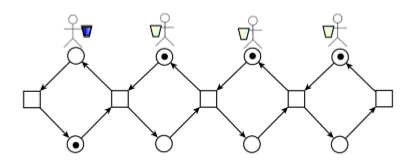
\includegraphics[width=0.7\textwidth]{img/reti/rete_spegnimento_fuoco.png}
    \caption{Esempio di una rete per modellare il sistema di spegnimento del fuoco}
    \label{fig:spegnimento-fuoco}
\end{figure}
\begin{definizione}[\textbf{Rete causale}]
    Definiamo $N = (B,E, F)$ come una \textbf{rete causale}, detta anche rete di
    occorrenze senza conflitti, se e solo se:
    \begin{itemize}
        \item $\forall b \in B: |^{\bullet}b| \leq 1 \land |b^{\bullet}| \leq 1$
              ovvero non si hanno conflitti; quindi, per ogni condizione si ha al più
              un pre-evento e un post evento. (Avendo quindi al più un arco entrante
              e al più uno uscente).
        \item $\forall x, y \in B \cup E: (x, y) \in F^{+} \Rightarrow (y, x) \notin F^{+})$
              ovvero non si hanno cicli; quindi, presi due elementi collegati da una
              sequenza di archi orientati, avendo un cammino tra i due elementi ($F^{+}$
              è la chiusura transitiva della relazione $F$) non ho anche un cammino
              opposto tra i due.
        \item $\forall e \in E: \{x \in B \cup E | xF^{\ast}e\}$ è finito, ovvero
              si ha un numero finito di pre-elementi di un certo elemento.
    \end{itemize}
    Sono quindi reti che registrano un comportamento e quindi non si hanno
    conflitti (che in caso sono sciolti registrando solo quello che è effettivamente
    successo e non quello che potrebbe succedere). Si registra una run del sistema.
    Non si hanno nemmeno cicli perché ogni ripetizione dell'evento viene concatenata
    a quella prima.

    La rete può essere quindi si infinita ma è composta da un insieme di elementi
    finito che si ripete. In ogni caso il passato di un evento è finito e registrato,
    anche se nel complesso il comportamento è infinito “in avanti”. Con una rete
    causale si possono non distinguere più condizioni ed eventi.
\end{definizione}
Ad una rete causale è possibile associare un \textbf{ordine parziale}:
\begin{equation}
    (X, \leq) = (B \cup E, F^{\ast})
\end{equation}
Dicendo che un elemento “è minore” di un altro se esiste un cammino orientato
dall'uno all'altro.
\begin{definizione}
    Data una rete causale $N = (B,E, F)$ e dato un ordine parziale $(X, \leq)$
    con $X = B \cup E$ si ha che si può interpretare la relazione d'ordine come
    indipendenza o dipendenza causale, ovvero presi $x, y \in X$ come elementi
    che occorrono nella storia di $X = B \cup E$ si hanno le seguenti diciture:
    \begin{itemize}
        \item $x \leq y$ (avendo un cammino da $x$ a $y$) corrisponde a $x$ causa
              $y$, ovvero si ha una relazione di dipendenza causale tra i due.
        \item $x \ \textbf{li} \ y$ indica che $x \leq y \lor y \leq x$ e quindi
              corrisponde a $x$ e $y$ sono causalmente dipendenti. Si ha che \textbf{li}
              può venire letto come linea ($x$ in linea con $y$) avendo che uno dei
              due precede l'altro.
        \item $x \textbf{co} \ y$ indica che: $\lnot(x < y)\  \land  \ \lnot (y < x)$
              e quindi corrisponde a $x$ e $y$ sono \textbf{causalmente indipendenti},
              avendo che i due elementi non si precedono a vicenda, non avendo ordine
              tra loro. Si ha che \textbf{co} sta per concurrency.
    \end{itemize}
    Le relazioni \textbf{li} e \textbf{co} sono riflessive e simmetriche ma non transitive.
\end{definizione}
\begin{definizione}
    Data una rete causale $N = (B,E, F)$ e dato un ordine parziale $(X, \leq)$
    con $X = B \cup E$ definiamo:
    \begin{equation}
        C \subseteq X
    \end{equation}
    come:
    \begin{itemize}
        \item \textbf{co-set} se e solo se $\forall x, y \in C$: $x \ \textbf{co} \ y$,
              quindi $C$ è una clique della relazione \textbf{co}.
        \item \textbf{taglio} se e solo se $C$ è un \textbf{co-set} massimale
              (tutti gli elementi nel taglio sono in relazione \textbf{co})
    \end{itemize}
    Definiamo $C$ come \textbf{co-set} massimale se e solo se $\forall y \in X \backslash C$
    si ha che:
    \begin{equation}
        \exists c \in C: y \textbf{li} \ c
    \end{equation}

    Definiamo:
    \begin{equation}
        L \subseteq X
    \end{equation}
    come:
    \begin{itemize}
        \item \textbf{li-set} se e solo se $\forall x, y \in L: \ x \ \textbf{li} \ y$
        \item \textbf{linea} se e solo se $L$ è un \textbf{li-set} massimale.
    \end{itemize}
    Definiamo $L$ come \textbf{li-set} massimale se e solo se $\forall y \in X
        \backslash L$ si ha che:
    \begin{equation}
        \exists l \in L: \ y \textbf{co}  \ l
    \end{equation}
    Si ha quindi che:
    \begin{itemize}
        \item In un \textbf{co-set} la relazione \textbf{co} è transitiva.
        \item In un \textbf{li-set} la relazione \textbf{li} è transitiva.
    \end{itemize}
    Tagli e linee possono essere fatti sia di condizioni che di eventi.
\end{definizione}
Un taglio $C \subseteq X$ è detto $B$-taglio se $C \subseteq B$.

I tagli fatti di sole condizioni rappresentano casi raggiungibili dal sistema.

Una rete causale, quindi, registra il comportamento di un sistema elementare. Si
hanno quindi, con i tagli, possibili osservazioni di configurazioni possibili
nella storia del sistema.
\begin{definizione}
    Grazie alle reti causali, preso un elemento $x \in X$, possiamo definire:
    \begin{itemize}
        \item $\textbf{past}(x)$, ovvero il passato dell'elemento, tutti gli
              elementi in relazione $\leq$ di $x$.
        \item $\textbf{future}(x)$, ovvero il futuro dell'elemento, tutti gli
              elementi in relazione $\geq$ di $x$.
    \end{itemize}
    Gli elementi nell'anti-cono sono in relazione \textbf{co} con $x$ e quindi
    possono essere concorrenti.
\end{definizione}
\begin{definizione}[\textbf{k-densità}]
    $N = (B, E, F)$ rete causale, $(X = (B \cup E), \leq)$ ordine parziale. Si
    ha che $N$ è \textbf{$k-$densa} se e solo se:
    \begin{equation}
        \forall h \in Linee(N), \ \forall c \in Tagli(N): \ |h \cap c| = 1
    \end{equation}
    dove $Linee(N)$ e $Tagli(N)$ sono gli insiemi delle linee e dei tagli di $N$.
\end{definizione}
\begin{nota}
    Se la rete causale $N$ è finita allora $N$ è anche $K-$densa.
\end{nota}
\begin{figure}[!ht]
    \centering
    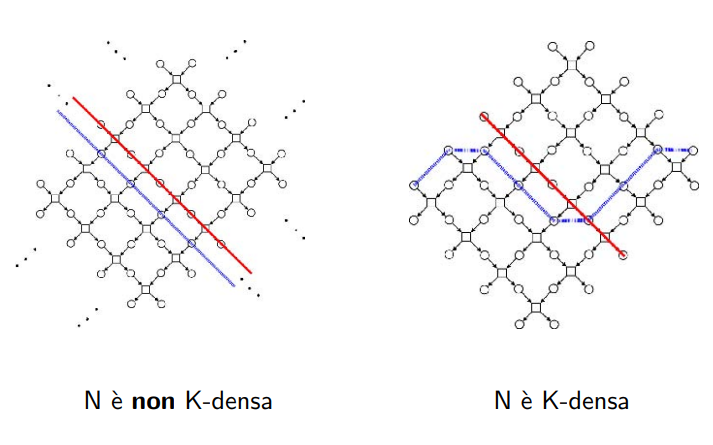
\includegraphics[width=0.7\textwidth]{img/reti/kdensa.png}
    \caption{Esempio di rete $K$-densa}
\end{figure}
\begin{definizione}[\textbf{Processi non sequenziali}]
    Sia $\Sigma = (S, T, F, c_{in})$ un sistema elementare senza contatti e finito,
    ovvero con $S \cup T$ finito.

    $\langle N = (B, E, F), \phi \rangle$ è un \textbf{processo non sequenziale}
    su $\Sigma$ se e solo se:
    \begin{itemize}
        \item $(B, E, F)$ è una rete causale nella quale si ammettono condizioni
              isolate.
        \item $\phi: B \cup E \to S \cup T$ è una mappa tale che:
              \begin{enumerate}
                  \item $\phi(B) \subseteq S, \ \phi(E) \subseteq T$
                  \item $\forall x_1, x_2 \in B \cup E: \ \phi(x_1) = \phi(x_2)
                            \Rightarrow (x_1 \leq x_2) \ \lor \ (x_2 \leq x_1)$
                  \item $\forall e \in E: \ \phi(^{\bullet}e) = ^{\bullet}\phi(e)
                            \ \land \ \phi(e^{\bullet}) = \phi(e)^{\bullet}$
                  \item $\phi(Min(N)) = c_{in}$ dove
                        $Min(N) = \{x \in B \cup E | \not\exists y: \ (y, x) \in F\}$
                        ovvero non hanno un arco entrante, sono gli stati locali
                        iniziali.
              \end{enumerate}
    \end{itemize}
\end{definizione}
Se $\langle N = (B, E, F); \phi \rangle$ è un processo non sequenziale di
$\Sigma = (S, T, F, c_{in})$ sistema elementare finito e senza contatti allora:
\begin{itemize}
    \item $N = (B, E, F)$ è $K$-densa
    \item $\forall K \subseteq B$, $K\ B$-taglio di $N$ è tale che: $K$ è finito e
          $\exists c \in C_{\Sigma}: \ \phi(K) = c$
\end{itemize}
I B-tagli corrispondono ai casi raggiungibili perché sono contemporaneamente veri.
\begin{nota}
    In sostanza per accorgersi subito se è un processo sequenziale allora:
    \begin{itemize}
        \item devono comparire tutti gli stati del caso iniziale
        \item se c'è un evento allora devono essere rappresentate tutte le sue 
        precondizioni e postcondizioni
        \item non ci devono essere conflitti nel processo non sequenziale
    \end{itemize} 
\end{nota}
\subsection{Reti di Occorrenze}
Vogliamo avere una struttura che registri tutti i comportamenti possibili
registrando le dipendenze e le indipendenze tra i processi. Posso avere una
struttura che mi raccolga tutti i possibili processi sequenziali.
\begin{definizione}[\textbf{Relazione di conflitto}]
    Una \textbf{relazione di conflitto}  $\#\subseteq (B\cup E)\times (B\cup E)$
    è definita come
    \begin{equation}
        x\#y\iff \exists e_1,e_2\in E :^{\bullet}e_1 \cap ^{\bullet} e_2\ne \emptyset
        \land e_1\le x \land e_2\le y
    \end{equation}
    due elementi sono in relazione se nel loro passato hanno 2 eventi in conflitto.
\end{definizione}
\begin{definizione}[\textbf{Rete di occorrenze}]
    $N = (B, E, F)$ è una \textbf{rete di occorrenze} se e solo se:
    \begin{itemize}
        \item \textbf{conflitti solo in avanti}: $\forall b \in B: \ | ^{\bullet}b|
                  \leq 1$ sono presenti dei conflitti solo in avanti.
        \item \textbf{aciclica}: $\forall x, y \in B \cup E: \ (x, y) \in F^{+}
                  \Rightarrow (y, x) \notin F^{+}$
              non ci sono cicli
        \item\textbf{passato finito}: $\forall e \in E: \{x \in B \cup E| \
                  xF^{\ast} e \}$ è finito
        \item \textbf{relazione di conflitto} $\#$ non è riflessiva.
    \end{itemize}
\end{definizione}
In queste reti è ancora possibile associare a $N$ un ordine parziale
$(X, \leq) = (B \cup E, F^{\ast})$:
\begin{itemize}
    \item $x \ \textbf{li} \ y$ sse $x\le y$ o $y\le x$
    \item $x \ \# \ y$ sse $\exists e_1,e_2\in E :^{\bullet}e_1 \cap ^{\bullet} e_2\ne \emptyset
    \land e_1\le x \land e_2\le y$
    \item $x \ \textbf{co} \ y$ sse $\lnot (x<y)$ e $\lnot (y<x)$ e $\lnot x\#y$
\end{itemize}

Se i due elementi non sono ordinati allora saranno o in relazione $co$ o in \textbf{conflitto}. 

\begin{nota}
    La proprietà 2 e 3 delle reti causali in and tra loro implicano la proprietà 3
    delle reti di occorrenze. Un ragionamento analogo può essere fatto per le proprietà
    2 e 4 delle reti causali, le quali in and implicano la proprietà 4 delle reti
    di occorrenza.
\end{nota}

\begin{nota}
    Un processo non sequenziale può essere definito anche richiedendo che $\phi$
    soddisfi: (1),(2),(3') e (4'), dove 3' e 4' implicano le proprietà 3 e 4
    delle reti di occorrenza.
\end{nota}
\begin{definizione}[\textbf{Processo ramificato}]
    Sia $\Sigma = (S,T, F, c_{in})$ un sistema elementare senza contatti e finito.
    $\langle N = (B, E, F); \phi \rangle$ è un \textbf{processo ramificato} di $\Sigma$
    se e solo se:
    \begin{itemize}
        \item $(B, E, F)$ è una rete di occorrenze (si ammettono condizioni isolate)
        \item $\phi: B \cup E \to S \cup T$ è una mappa:
              \begin{enumerate}
                  \item $\phi(B) \subseteq S, \ \phi(E) \subseteq T$
                  \item $\forall e_1, e_2 \in E: \ ( ^{\bullet} e_1 =  ^{\bullet}
                            e_2 \ \land \ \phi(e_1) = \phi(e_2)) \Rightarrow e_1 = e_2$
                  \item $\forall e \in E$ : la restrizione di $\phi$ a $^{\bullet} e$
                        è una biiezione tra $^{\bullet} e \ \text{e} \ ^{\bullet} \phi(e)$
                        e la restrizione di $\phi$ a $e^{\bullet}$ è una biiezione tra
                        $e^{\bullet} \ \text{e} \ \phi(e)^{\bullet}$
                  \item La restrizione di $\phi$ a $Min(N)$ è una biiezione tra
                        $Min(N)$ e $c_{in}$.
              \end{enumerate}
    \end{itemize}
\end{definizione}
\begin{definizione}[\textbf{Prefisso}]
    Sia $\Sigma = (S,T, F, c_{in})$ un sistema elementare finito e senza contatti
    e siano $\Pi_1 = \langle N_1; \phi_1 \rangle$, $\Pi_2 = \langle N_2; \phi_2 \rangle$
    processi ramificati di $\Sigma$.

    Allora $\Pi_1 = \langle N_1; \phi_1 \rangle$ è un \textbf{prefisso} di
    $\Pi_2 = \langle N_2; \phi_2 \rangle$ se e solo se $N_1$ è una sottorete di
    $N_2$ e $\phi_{2|N_1} = \phi_1$ ($\phi_2$ ”ristretto” a $N_1$ è uguale a $\phi_1$).
\end{definizione}

\begin{nota}
    Il prefissi di un processo ramificato sono i processi sequenziali finiti del
    del sistema elementare.
\end{nota}

\begin{definizione}[\textbf{Unfolding}]
    $\Sigma$, sistema elementare, ammette un unico processo ramificato che è massimale rispetto alla
    relazione di prefisso tra processi. Tale processo massimale è chiamato
    \textbf{unfolding} di $\Sigma$, denotato $Unf (\Sigma)$.
\end{definizione}
\begin{definizione}[\textbf{Corsa}]
    Un processo non sequenziale è un processo ramificato $\Pi = \langle N; \phi \rangle$
    tale che $N$ sia una rete causale (senza conflitti), tale processo è chiamato
    anche \textbf{corsa} (\textbf{run}).
\end{definizione}
\begin{osservazione}
    Inoltre, ogni processo non sequenziale di $\Sigma$ è un prefisso dell'unfolding
    $Unf (\Sigma)$.
\end{osservazione}

\section{Sistemi elementari - reti P/T- Reti ad alto livello}
Se dovessimo usare le reti elementari per modellare sistemi veri, avremmo
un'esplosione di condizioni ed eventi. Una rappresentazione più compatta è data
dalle \textbf{reti Posti e Transizioni} che utilizzano, invece delle condizioni
booleane dei sistemi elementari, dei contatori.
\begin{definizione}[\textbf{Sistema Posti e Transizioni}]
    Formalmente un sistema posti e transizioni è definito come:
    \begin{equation}
        \sigma = (S, T, F, K, W, M_0)
    \end{equation}
    dove:
    \begin{itemize}
        \item $(S, T, F)$ è una rete.
        \item \textbf{funzione capacità degli stati}: $K: S \to \mathbb{N}^+ \cup \{\infty\}$ è la funzione che assegna ai
              posti le capacità
        \item \textbf{funzione peso degli archi}: $W: F \to \mathbb{N}$ è la funzione peso degli archi
        \item \textbf{funzione di marcatura iniziale}: $M_0: S \to \mathbb{N}: \forall s \in S$ $M_0(s) \leq K(s)$ è la
              marcatura iniziale. È importante osservare che il numero di marche è sempre
              minore o uguale alla capacità del posto
    \end{itemize}
\end{definizione}
Ad esempio, pensiamo ad un buffer a due posizioni, nei sistemi elementari avremmo
due condizioni con due eventi deposita e preleva. Nei sistemi P/T possiamo usare
un contatore come fosse un'unica condizione. Chiaramente si perde dell'informazione,
in particolare non sappiamo più in quale posizione del buffer il produttore
deposita e da quale posizione il consumatore consuma.

Questa tipologia di reti mi permette di definire degli archi pesati, archi con
associato un numero, che abilitino o meno le transizioni.

Le reti ad alto livello, anche dette \textbf{reti colorate}, permettono di
ristabilire l'informazione persa con le reti Posti e transizioni assegnando una
struttura dati alle marche. Addirittura, una marca potrebbe rappresentare un
processo a sé stante.
\begin{definizione}[\textbf{Regola di scatto}] 
    Data la \textbf{marcatura} $M:S\to \mathbb{N}$ e una transizione $t\in T$:
    \begin{equation}
        M[t > \ \text{se e solo se} \ \forall s \in S \ M(s) \geq W(s, t) \ \land
        \ M(s) \ + \ W(t, s) \leq K(s)
    \end{equation}
    \begin{equation}
        M[t > M' \ \text{se e solo se} \ M[t > \ \land \ \forall s \in S \ M'(s)
        = M(s) - W(s, t) + W(t, s)
    \end{equation}
\end{definizione}
\begin{definizione}
    $\Sigma = (S,T,F,K,W,M_0)$ un \textbf{sistema} $P/T$, l'insieme delle
    \textbf{marcature raggiungibili} di $\Sigma$ è $[M_0>$, il più piccolo
    insieme tale che:
    \begin{itemize}
        \item $M_0\in [M_0>$
        \item $M\in [M_0>\land \exists t\in T: M[t>M'\implies M' \in [M_0>$
    \end{itemize}
\end{definizione}
\begin{definizione}
    $\Sigma = (S,T,F,K,W;M_0)$ un \textbf{sistema} $P/T$ allora
    $RG(\Sigma)=([M_0>,U_\Sigma,A,M_0)$ è il \textbf{grafo di raggiungibilità}
    di $\Sigma$, dove
    \begin{equation}
        S=\left\{(M,U,M'):M,M'\in [M_0>\land U\in U_\Sigma\land M[U>M' \right\}
    \end{equation}
\end{definizione}
Anche qui, come nei sistemi elementari si può costruire l'insieme delle marcature
raggiungibili e il relativo grafo di raggiungibilità. Generalmente in queste reti
la Diamond property non è più valida, questo causa self-loop.

Anche per le reti P/T si possono avere dei contatti, ovvero, situazioni in cui 
il peso dell'arco è $w$, la capacità del nodo di arrivo $k$ e la sua marcatura è
$m_s\ne 0$ allora ho un \textbf{contatto} se $w+m_s >k$. Quindi non può scattare
la regola visto che dovrebbero passare $w$ marche allo stato $s$ ma quest'ultimo
ha già $m_s$ marche ed aggiungendone altre si supera il vincolo sulla capacità 
del nodo.  

Come per i sistemi elementari, anche nelle reti a P/T è possibile aggiungere stati (quindi posti)
per eliminare situazione di \textbf{contatto}. In sostanza si aggiungono per ogni 
stato la versione \textbf{complementata} e questo permette di eliminare il vincolo sulla capacità,
senza alterare il comportamento del sistema.
\begin{definizione}
    Un sistema $P/T$ $\Sigma = (S,T,F,K,W;M_0)$ è \textbf{senza contatti} sse
    $\forall M\in [M_0>,\forall t\in T, \forall s\in S$:
    \begin{equation}
        M(s)\ge W(s,t)\implies M(s)+W(t,s)\le K(s)
    \end{equation}
\end{definizione}
Se $\Sigma = (S,T,F,K,W;M_0)$ è un \textbf{sistema} $P/T$ senza contatti allora
$t$ è \textbf{abilitata} in $M\in [M_0>$ ($M[t>$) sse
\begin{equation}
    \forall s\in S, M(s)\ge W(s,t)
\end{equation}
Nei sistemi senza contatti la \textbf{capacità} non ha alcun ruolo nella regola
di scatto perché la transizione può scattare se nei suoi posti di input ci sono
abbastanza marche.
\begin{definizione}[\textbf{Reti marcate}]
    Un sistema Posti e transizione è una \textbf{rete marcata} se non ha vincoli sulla
    capacità dei posti e ha tutti gli archi di peso unitario.
    \begin{equation}
        \forall s\in S, M_0(s)\in \mathbb{N}\land K(s)=\infty \land \forall t\in
        T, W(s,t)\le 1\land W(t,s)\le 1
    \end{equation}
    Le reti marcate sono denotate da $(S,T,F;M_0)$ in quanto $K,W$ sono ridondanti
\end{definizione}

\begin{definizione} [\textbf{Reti marcate sicure}]
    $\Sigma = (S,T,F;M_0)$ una \textbf{rete marcata} allora è \textbf{sicura}
    (\textbf{safe}) sse:
    \begin{equation}
        \forall M\in [M_0>,\forall s\in S:M(s)\le1
    \end{equation}
\end{definizione}
Una rete marcata è \textbf{safe} se comunque evolva il comportamento avremmo in
ogni posto sempre al più una marca, i posti hanno quindi $0$ o $1$ marca e possiamo
interpretarli di nuovo come condizioni booleane. L'unica differenza con le reti
elementari è che nelle reti safe i cappi sono abilitati, mentre nelle reti
elementari questo non succede. Se eliminiamo i cappi dalle reti marcate safe,
otteniamo il corrispettivo di un sistema elementare puro.

\begin{definizione}
    Sia $\Sigma = (S,T,F,K,W;M_0)$ è un \textbf{sistema} $P/T$ tale che
    $\forall s\in S,K(s)=\infty$ e $N=(S,T,F)$ è \textbf{senza cappi}. Allora il
    sistema può essere rappresentato da un'unica matrice $\underline{N}:S\times
        T\rightarrow\mathbb{N}$
    chiamata \textbf{matrice di incidenza}.
\end{definizione}
Quindi avremo che
\begin{equation}
    M_0[t_1>\iff \underline{M_0}+\underline{t_1}\ge \underline{0} (\iff
    \underline{M_0}+\underline{N_{t_1}}\ge \underline{0})
\end{equation}
Quindi ogni cambio di stato lo possiamo codificare con una somma di vettori colonna,
utilizzando l'\textbf{equazione di stato}:
\begin{equation}
    M_0[\sigma>M_1\implies \underline{M_0}+\underline{N}\cdot \underline{c_\sigma}
    =\underline{M_1}
\end{equation}

\begin{esempio}
    Supponiamo di avere la seguente rete P/T.
    \begin{figure}
        \centering
        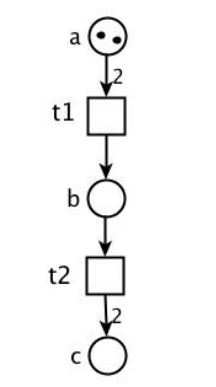
\includegraphics[width=0.2\textwidth]{img/reti/EsercizioP-T.png}
    \end{figure}
    Iniziamo a calcolare la matrice di incidenza calcolando ogni singola cella 
    in questo modo:
    $$N[s,t]= \begin{cases}
        - W(s,t)& (s,t)\in F\\
        W(s,t)& (t,s)\in F
    \end{cases}$$
    Quindi in questo caso la tabella sarà
    \begin{equation}
        \begin{array}{|c|c|c|}
            \hline
              &t_1&t_2\\
            \hline
            a & -2 & \\
            b & 1 & -1\\
            c &   & 2\\
            \hline
        \end{array}
    \end{equation}
    Successivamente calcolo le singole marcature in questo modo:
    $$M_1 = M_0 + t_1 \ \ \ M_2 = M_1 + t_2 $$
    \begin{equation}
        \begin{array}{|c|c|c|c|}
            \hline
              &M_0&M_1&M_2\\
            \hline
            a & 2 &  &\\
            b &  & 1 &\\
            c &   &  & 2\\
            \hline
        \end{array}
    \end{equation}
    Si possono anche eseguire in sequenza utilizzando l'equazione di stato e quindi
    calcolare in un solo passo la marcatura di una sequenza di transizioni (aspetta risposta)
\end{esempio}

\begin{osservazione}
    Sia $\Sigma = (S,T,F,K,W,M_0)$ un \textbf{sistema} $P/T$ tale che $\forall s
        \in S, K(s)=\infty$:
    \begin{itemize}
        \item $\Sigma$ è \textbf{limitato} sse $\exists n\in \mathbb{N}: \forall
                  s\in S, \forall M\in [M_0>$:
              $$M(s)\le n$$
        \item $\Sigma$ è \textbf{safe} sse $$\forall s\in S, \forall M\in
                  [M_0> \ : \ M(s)\le 1$$
        \item
              $\Sigma$ è \textbf{limitato} $\iff [M_0>$ è un insieme \textbf{finito}
              ($RG(\Sigma)$ è \textbf{finito}).
        \item $\Sigma$ è \textbf{terminante} sse non ammette sequenze infinite
        \item $M\in [M_0>$ è una marcatura di \textbf{deadlock} sse $\forall t\in
                  T,\lnot(M[t>)$
        \item $\Sigma$ è \textbf{deadlock-free} sse $\forall M\in[M_0>\exists t\in
                  T:M[t>$
              $$(\iff \not\exists M\in [M_0>:M\text{ è una marcatura di deadlock})$$
        \item $\Sigma$ è $1$\textbf{-vivo} sse
              $$\forall t\in T,\exists M\in [M_0>:M[t>$$
        \item  $\Sigma$ è \textbf{vivo} sse
              $$\forall t\in T,\forall M\in [M_0>,\exists M'\in [M>:M'[t>$$
              \textbf{vivezza} $\implies$ assenza di \textbf{deadlock}.
        \item $\Sigma$ è \textbf{reversiblile} (ciclico) sse
              $$\forall M\in [M_0>:M_0\in [M>$$
        \item $\Sigma$ è \textbf{reversibile} $\iff$ il suo grafo delle marcature
              raggiungibili è \textbf{strettamente connesso}
        \item reversibilità $+ 1$-vivezza$\implies$ vivezza
    \end{itemize}
\end{osservazione}

Per verificare le proprietà allora si può fare:
\begin{itemize}
    \item analisi del grafo di raggiungibilità o di un prefisso dell'unfolding
    \item analisi strutturale del grafo della rete:
          \begin{itemize}
              \item tecniche che sfruttano l'algebra lineare come le \textbf{equazioni
                        di stato} che descrivono la dinamica e le $S$-invarianti
                    e le $T$-invarianti
              \item studio del grafo della rete come sottoinsiemi di nodi...
              \item controllo delle condizioni necessarie e sufficienti per alcune
                    sottoclassi di reti.
          \end{itemize}
\end{itemize}


\subsection{Reti ad alto livello}
Dal momento che le reti P/T hanno un problema di perdita di informazioni, allora
si può risolvere modellando le marche (contatori) con una struttura dati.
\chapter{Dimostrazioni di correttezza}
\section{Logica proposizionale}
Nella logica proposizionale, dal punto di vista teorico, il significato di una
formula è rappresentato dal suo valore di verità.

Una volta definite sintassi e semantica, possiamo usare una logica per costruire
delle dimostrazioni. Aver definito una semantica non vuol dire che di fronte ad
una formula si è in grado di dire subito se sia valida o meno, dunque con la logica
si sviluppa un metodo di dimostrazione e si cerca, in un numero finito di passi,
di dimostrare la validità di una certa formula.

Un esempio, legato alla logica dell'aritmetica, è la formula che dice che per ogni
numero primo, esiste sempre un numero primo più grande di esso; questa formula
non è verificabile sperimentalmente essendo in numeri infiniti e va quindi
dimostrata in altri modi.

Per ogni logica bisogna quindi definire un apparato deduttivo, cioè un insieme di
\textbf{regole di inferenza}. Una regola di inferenza è una regola che dice "se
hai già dimostrato queste premesse, allora puoi dedurre questa formula".
\subsection{Sintassi}
Passiamo ora al caso specifico della logica proposizionale che ci servirà per le
dimostrazioni di correttezza.

Per costruire il linguaggio avremmo bisogno di:
\begin{itemize}
    \item $PA = \{p_1, \dots, pi, \dots\}$ sono le proposizioni atomiche.
    \item $\bot, \ \top$ sono le costanti logiche, rappresentano formule o sempre
          false o sempre vere.
    \item $\lnot, \ \land, \ \lor, \ \implies, \ \iff$ sono i connettivi logici,
          utilizzati per creare formule complesse.
    \item $(, \ )$ sono i delimitatori, utilizzati per la creazione di formule
          complesse.
\end{itemize}
Adesso dobbiamo definire la grammatica della logica proposizionale, per fare ciò
si utilizza una definizione induttiva.
\begin{definizione}[\textbf{Formule ben formate}]
    Definiamo l'insieme delle formule ben formate $FbF_p$ come:
    \begin{itemize}
        \item $\bot, \ \top \in FbF_p$ le costanti logiche sono delle formule ben
              formate.
        \item $\forall p_i \in PA, \ p_i \in FbF_p$ le proposizioni atomiche sono
              formule ben formate.
        \item Se $A, B \in FbF_p$ allora:
              \begin{equation}
                  (\lnot A), \ (A \land B), \ (A \lor B), \ (A \implies B), \
                  (A \iff B) \ \in FbF_p
              \end{equation}
        \item Nient'altro è una formula ben formata.
    \end{itemize}
\end{definizione}
Le formule atomiche rappresentano delle relazioni tra le variabili e le costanti
oppure relazioni tra le variabili.
\subsection{Semantica}
Siamo ora interessati a conoscere il valore di una formula scritta attraverso la
logica proposizionale. Il \textbf{valore di verità} di una formula dipende dai
valori di verità delle sue proposizioni atomiche.

Il punto di partenza è quindi stabilire quali proposizioni atomiche sono da
considerare vere. Questo si può fare formalmente definendo una \textbf{funzione
    di valutazione}:
\begin{equation}
    v: PA \to \{0, 1\}
\end{equation}
I connettivi della logica proposizionale hanno i seguenti valori di verità:
\begin{equation}
    \begin{array}{ccccccc}
        \toprule
        A & B & A \land B & A \lor B & \lnot A & A \implies B & A \iff B \\
        \midrule
        F & F & F         & F        & T       & T            & T        \\
        F & T & F         & T        & T       & T            & F        \\
        T & F & F         & T        & F       & F            & F        \\
        T & T & T         & T        & F       & T            & T        \\
        \bottomrule
    \end{array}
\end{equation}
Questa funzione di valutazione può essere estesa induttivamente ad una funzione
definita su tutte le formule ben formate, tale funzione prende il nome di
\textbf{funzione di interpretazione} ed è definita come:
\begin{equation}
    I_v: FbF_p \to \{0, 1\}
\end{equation}
\begin{enumerate}
    \item $I_v (\bot) = 0$ e $I_v (\top) = 1$ le costanti logiche hanno valore
          di verità definito.
    \item $\forall p_i \in PA, \ I_v(p_i) = v(p_i)$ l'interpretazione di una
          preposizione atomica è data dal suo valore di verità.
    \item Passo induttivo:
          \begin{equation}
              \begin{array}{cc}
                  I_v(\lnot A) = 1 - I_v(A) &                                  \\
                  I_v(A \lor B) = 1         & \text{se e solo se} \ I_v(A) = 1
                  \ \text{o} \ I_v(B) = 1                                      \\
                  \dots                     &                                  \\
                  I_v(A \to B) = 1          & \text{se e solo se} \ I_v(A) = 0
                  \ \text{o} \ I_v(B) = 1
              \end{array}
          \end{equation}
\end{enumerate}
Vediamo ora un po' di terminologia:
\begin{itemize}
    \item $A$ è \textbf{soddisfatta} da $I_v$ se $I_v(A) = 1$.
    \item $A$ è \textbf{soddisfacibile} se esiste $I_v$ tale che $I_v(A) = 1$.
    \item $A$ è una \textbf{tautologia} se $I_v(A) = 1$ per ogni $I_v$.
    \item $A$ è una \textbf{contraddizione} se $I_v(A) = 0$ per ogni $I_v$.
\end{itemize}
\begin{definizione}[\textbf{Logicamente equivalenti}]
    Due formule ben formate $A$ e $B$ sono logicamente equivalenti allora:
    \begin{equation}
        A \equiv B \iff I_v(A) = I_v(B), \ \forall I_v
    \end{equation}
\end{definizione}
Si possono definire le seguenti \textbf{equivalenze logiche}:
\begin{itemize}
    \item $A \land (A \lor B) \equiv A$
    \item $\lnot (\lnot A) \equiv A$
    \item $\lnot (A \land B) \equiv \lnot A \lor \lnot B$
    \item $A \lor \lnot A \equiv \top$
    \item $A \implies B \equiv \lnot B \implies \lnot A$
    \item $A \land \lnot A \equiv \bot$
\end{itemize}
Definiamo ora i modelli, ovvero delle interpretazioni delle proposizioni
atomiche, cioè una scelta di valori di verità per tutte le proposizioni atomiche.
\begin{definizione}[\textbf{Modello}]
    Un \textbf{modello} è un sottoinsieme delle proposizioni atomiche $M
        \subseteq PA$ a cui è associata un'interpretazione definita come $I_M:
        FbF_p \to \{0, 1\}$ tale che:
    \begin{equation}
        I_M(p_i) = 1 \ \text{se e solo se} \ p_i \in M
    \end{equation}
    Possiamo indicare la relazione tra modelli e formule come:
    \begin{equation}
        M \models A
    \end{equation}
    la quale si può leggere come $M$ modella $A$ oppure come $A$ è soddisfatta
    in $M$. Quindi scriveremo $M \models A$ se $A$ risulta vera per la scelta
    particolare di $M$.
\end{definizione}
\begin{definizione}[\textbf{Tautologia}]
    Se $M \models A$ per tutti gli $M$, allora $A$ è una tautologia e si indica
    $\models A$.
\end{definizione}
\begin{definizione}[\textbf{Soddisfacibilità}]
    Se $M \models A$ per qualche $M$, allora $A$ è soddisfacibile.
\end{definizione}
\begin{definizione}[\textbf{Insoddisfacibilità}]
    Se $M \models A$ non è soddisfatta da nessun $M$, allora $A$ è insoddisfabile.
\end{definizione}
\subsection{Apparato deduttivo}
Possiamo ora rappresentare l'apparato deduttivo della logica proposizionale. Esso
è composto da \textbf{regole di inferenza} scritte in questo modo:
\begin{equation}
    \frac{A_1, \dots, A_n}{B}
\end{equation}
dove $A_i \in FbF_p$ sono le \textit{premesse}, mentre $B \in FbF_p$ è la
\textit{conclusione}.

Alcune regole di inferenza sono ad esempio:
\begin{itemize}
    \item Se ho dimostrato che $A_1$ e $A_2$ sono vere, sarà vera anche $A_1
              \land A_2$:
          \begin{equation}
              \frac{A_1 \ \ A_2}{A_1 \land A_2}
          \end{equation}
    \item Se ho dimostrato che $A_1 \land A_2$ è vera, sarà vera anche $A_1$:
          \begin{equation}
              \frac{A_1 \land A_2}{A_1}
          \end{equation}
    \item Modus Ponens:
          \begin{equation}
              \frac{A \ \ A \implies B}{B}
          \end{equation}
    \item Modus Tollens:
          \begin{equation}
              \frac{A \implies B \ \ \lnot B}{\lnot A}
          \end{equation}
\end{itemize}
Le regole di inferenza sono la base da cui è possibile costruire le dimostrazioni.
\begin{definizione}[\textbf{Dimostrazione}]
    Una \textbf{dimostrazione} è definita come una catena di regole $A_1, \dots,
        A_n \vdash B$, ovvero da $A_1, \dots, A_n$ si deriva $B$.
\end{definizione}
Abbiamo ora due nozioni distinte:
\begin{itemize}
    \item La validità in un modello $\models$.
    \item La derivabilità $\vdash$ introdotta perché in generale non siamo in
          grado di decidere direttamente la nozione semantica di validità e
          quindi cerchiamo di dimostrare una cosa.
\end{itemize}
\begin{teorema}[\textbf{Validità, Correttezza}]
    Se $A_1, \dots, A_n \vdash B$ allora $A_1, \dots, A_n \models B$. Ovvero, se
    riusciamo a derivare $B$ da $A_1, \dots, A_n$ in ogni modello in cui sono
    vere $A_1, \dots, A_n$ allora è vera anche $B$.
\end{teorema}
Questo teorema ci dice che abbiamo scelto bene le regole di inferenza e che
queste non ci permettono di derivare cose non vere. Se questo teorema è valido,
la logica è corretta.
\begin{teorema}[\textbf{Completezza}]
    Se $A_1, \dots, A_n \models B$ allora $A_1, \dots, A_n \vdash B$, ovvero se
    in ogni modello in cui sono vere $A_1, \dots, A_n$ ed è soddisfatta anche
    $B$, si può derivare $B$ da $A_1, \dots, A_n$.
\end{teorema}
Questo teorema ci dice che possiamo dimostrare tutto ciò che è vero. Se questo
teorema è valido, la logica è completa.
\section{Logica di Hoare}
Questa logica si può vedere come costruita su due livelli diversi poiché permette
di stabilire e definire il criterio di correttezza per un dato programma.
In particolare, definisce questa correttezza tramite le definizioni di
\textit{precondizioni} e \textit{post-condizioni} rappresentate da formule della
logica proposizionale.
\subsection{Primo livello}
Al primo livello avremmo le proposizioni atomiche definite come relazioni fra le
variabili del programma, tra queste relazioni possiamo trovare anche relazioni
tra le variabili e le costanti.

Per dare una semantica, alle varie proposizioni atomiche definiamo la nozione di
\textbf{stato della memoria}.
\begin{definizione}[\textbf{Stato di memoria}]
    Sia $V$ l'insieme delle variabili del programma, definiamo uno \textbf{stato
        della memoria} come una fotografia della memoria del programma in un
    certo istante.

    Possiamo definire più formalmente quest'idea di stato della memoria come una
    funzione definita dall'insieme delle variabili ai numeri interi che assegna
    un valore ad ogni variabile.
    \begin{equation}
        \sigma: V \to \mathbb{Z}
    \end{equation}
    Diremo quindi che la formula $\alpha$ è vera in $\sigma$ scrivendo $\sigma
        \models \alpha$
\end{definizione}
\subsection{Secondo livello}
Le formule della logica di Hoare sono costruite tramite delle triple che prendono
il nome di triple di Hoare, le quali sono definite come:
\begin{equation}
    \{\alpha\} \ C \ \{\beta\}
\end{equation}
dove:
\begin{itemize}
    \item $\{\alpha\}$: è una formula che rappresenta le precondizioni.
    \item $C$: rappresenta un programma o un comando.
    \item $\{\beta\}$: è una formula che rappresenta le post-condizioni.
\end{itemize}
Le triple di Hoare si leggono come segue:
\begin{center}
    Se il comando $C$ viene eseguito a partire da uno stato della memoria nel
    quale $\alpha$ è vera, allora l'esecuzione termina e nello stato finale
    $\beta$ è vera.
\end{center}
\subsection{Linguaggio}
Definiamo ora il linguaggio che useremo con le triple di Hoare:
\begin{itemize}
    \item Espressioni aritmetiche $E$ definite come:
          \begin{itemize}
              \item Se $z \in \mathbb{Z}$ allora $z$ è un'espressione aritmetica
                    $z \in E$.
              \item $\forall e_1, e_2 \in E$ allora: $(e_1 + e_2), (e_1 - e_2),
                        - e_1, (e_1 \ast e_2), (e_1 / e_2), (e_1 \% e_2) \in E$
          \end{itemize}
    \item Espressioni logiche $B$ definite come:
          \begin{itemize}
              \item Le costanti logiche $true$ e $false$ sono espressioni logiche
                    $true, \ false \in B$.
              \item $\forall b_1, b_2 \in B$ allora: $ (b_1 \& b_2), (b_1 | b_2),
                        !b_1 \in B$
              \item $\forall e_1,e_2\in E$ allora $(e_1 < e_2), (e_1 == e_2),
                        (e_1 != e_2 ), (e_1 <= e_2) \in B$
          \end{itemize}
    \item Comandi $C$ definiti come:
          \begin{itemize}
              \item $\text{skip} \in C$ questa istruzione non modifica la memoria.
              \item Assegnamento $v := e \ \in C$ dove $v$ è una variabile ed $e$
                    è un espressione aritmetica.
              \item Operatore di sequenza $C, D \ \in C $ dove $C$ e $D$ sono dei
                    comandi.
              \item Operatore di scelta $\text{if} \ B \ \text{then} \ C \
                        \text{else} \ D \ \text{endif} \ \in C$ dove $B$ è un
                    espressione logica, mentre $C, D$ è sono dei comandi.
              \item Operatore di iterazione $\text{while} \ B \ \text{do} \ C \
                        \text{endwhile}$ dove $B$ è un espressione logica
                    e $C$ è un comando.
          \end{itemize}
\end{itemize}
possiamo estendere il linguaggio introducendo altri comandi e strutture:
\begin{itemize}
    \item do-while: $\ \text{do} \ C \ \text{while} \ B \ \text{endwhile} \
              \equiv \ C; \ \text{while} \ B \ \text{do} \ C \ \text{endwhile}$
    \item repeat: $ \ \text{repeat} \ C \ \text{until} \ B \ \text{endrepeat} \
              \equiv \ C; \ \text{while} \ \lnot B \ \text{do} \ C \ \text{endwhile} $
    \item for: $ \ \text{for} \ (D;B;F) \ C \ \text{endfor} \equiv D;
              \text{while} \ B \ \text{do} \ C; F \ \text{endwhile}$
    \item procedure
    \item array
\end{itemize}
Una tripla di Hoare rappresenta un criterio di correttezza del programma, la sua
regola di derivazione è definita come:
\begin{equation}
    \frac{T_1, \dots, T_m, f_1, \dots, f_n}{T}
\end{equation}
dove al numeratore sono specificate le premesse che possano contenere sia triple
$T_i$ che formule ben formate $f_i$, mentre al denominatore troviamo la conclusione
che è una tripla $T$.

Vediamo ora come definire le regole di derivazione per i comandi introdotti:
\begin{enumerate}
    \item \textbf{Skip}:
          \begin{equation}
              \frac{}{\{p\} \text{ skip } \{p\}}
          \end{equation}
          in questo caso la premessa è vuota e, visto che con questa operazione
          non modifico lo stato della memoria, le pre-condizioni e le
          post-condizioni sono le stesse.
    \item \textbf{Sequenza}:
          \begin{equation}
              \frac{\{p\} \text{ C } \{p'\} \ \ \{p'\} \text{ D } \{q\}}{\{p\}
                  \text{ C; D } \{p\}}
          \end{equation}
          se le post-condizioni di C e le pre-condizioni di D sono le stesse
          posso mettere in sequenza i comandi ottenendo lo stesso risultato.
    \item \textbf{Scelta}:
          \begin{equation}
              \frac{\{p \land B\} \text{ C } \{q\} \ \ \{p \land \lnot B\}
                  \text{ D } \{q\}}{\{p\} \text{ if B then C else D endif } \{q\}}
          \end{equation}
          Se dimostriamo che:
          \begin{itemize}
              \item Eseguendo $C$ da uno stato dove vale la precondizione $p$ e
                    vale anche la condizione $B$ al termine dell'esecuzione vale
                    $q$.
              \item Eseguendo $D$ da uno stato dove vale $p$ ma non vale $B$
                    arriviamo comunque ad uno stato dove vale $q$.
          \end{itemize}
          Possiamo derivare la regola della scelta dove prima dell'esecuzione
          dell'$if$ vale $p$ mentre dopo vale $q$.
    \item \textbf{Implicazione} o \textbf{Conseguenza}:
          \begin{equation}
              \frac{p \to p' \ \ \{p'\} \text{ C } \{q\}}{\{p\} \text{ C } \{q\}}
          \end{equation}
          inoltre:
          \begin{equation}
              \frac{\{p\} \text{ C } \{q\} \ \ q \to q'}{\{p\} \text{ C } \{q'\}}
          \end{equation}
          Generalizzando possiamo dire che se abbiamo dimostrato una tripla e
          osserviamo una condizione che implica la precondizione della tripla,
          possiamo derivare la tripla con la condizione osservata al posto della
          precondizione. Discorso analogo è valido anche per la post-condizione.
    \item \textbf{Assegnamento}:
          \begin{equation}
              \frac{}{\{q[E/q]\} \text{ x } := \text{ E }\{q\}}
          \end{equation}
          dove con $q[E / x]$ indico il fatto che sostituisco ogni occorrenza di
          $x$ in $q$ con $E$.
    \item \textbf{Iterazione} (correttezza parziale):
          \begin{equation}
              \frac{\{inv \land B\} \text{ C } \{inv\}}{\{inv\} \text{ while } B
                  \text{ do C endwhile } \{inv \land \lnot B\}}
          \end{equation}
          l'idea per le istruzioni iterative è di trovare una formula che sia
          \textbf{invariante} rispetto al blocco dell'istruzione iterativa. Se
          troviamo un'invariante possiamo dire che se questa formula è vera
          all'inizio dell'istruzione iterativa, lo sarà anche alla fine e in più
          possiamo dire che al termine del blocco iterativo vale anche la
          negazione della condizione di ciclo.

          In generale, avendo un'istruzione $W = \text{ while B do C endwhile }$,
          se deriviamo $\vdash \{p \land B\} C \{p\}$, allora possiamo dire che
          $p$ è invariante rispetto a $W$.

          Data un'istruzione iterativa, non c'è un solo invariante. Ad esempio,
          $True$ è invariante per ogni istruzione iterativa. Generalmente ci
          interessano gli invarianti utili alla dimostrazione in corso. Nella
          pratica, le istruzioni iterative sono inserite in programmi, di
          conseguenza la scelta dell'invariante dipende dal contesto e si abbina
          alla regola dell'implicazione.

          A volte l'invariante non è assoluto, ma lo diventa aggiungendoci la
          condizione di ciclo. L'invariante in genere è violato guardando lo
          stato della memoria durante l'esecuzione del blocco, ma viene
          ripristinato al termine del blocco.
\end{enumerate}
\begin{definizione}[\textbf{Invariante di un ciclo}]
    Possiamo definire l'\textbf{invariante di un ciclo} come una formula che se
    risulta vera all'inizio di un iterazione è vera anche alla fine di essa.
\end{definizione}
La logica di Hoare è una logica \textbf{corretta}, ovvero vale:
\begin{equation}
    \vdash \ \implies \ \models
\end{equation}
questo significa che tutte le triple che riusciamo a derivare sono sicuramente
delle triple valide. Inoltre, è anche \textbf{completa} (relativamente):
\begin{equation}
    \models \implies \vdash
\end{equation}
tutto ciò che è valido è derivabile. Tuttavia è una completezza relativa a causa
dell'incompletezza dell'aritmetica: potrebbe succedere di dover dimostrare una
proprietà aritmetica che però è indimostrabile (caso molto remoto).

Come notazione usiamo che:
\begin{equation}
    \vdash \{p\} \text{ C } \{q\}
\end{equation}
dove $\vdash$ segnala che la tripla è stata dimostrata con le regole di
derivazione (si parla quindi di sintassi, viene infatti ignorato il significato
ma si cerca solo di applicare le regole, ottenendo la conclusione come risultato
di una catena di regole).

Usiamo anche:
\begin{equation}
    \models \{p\} \text{ C } \{q\}
\end{equation}
dove $\models$ indica che la tripla è vera (si parla quindi di semantica,
riferendosi al significato).

Dato che si ha completezza e correttezza dell'apparato deduttivo si hanno due
situazioni.
\begin{itemize}
    \item Ogni tripla derivabile è anche vera in qualsiasi interpretazione.
    \item Ogni tripla vera vorremmo fosse anche derivabile e il discorso verrà
          approfondito in seguito per la logica di Hoare
\end{itemize}
\begin{nota}
    Negli esercizi si assegna a $\vdash$ una sigla, posizionata come pedice o
    apice, per rappresentare la regola che viene applicata.
\end{nota}
\subsection{Correttezza totale}
Vogliamo ora analizzare la correttezza totale dell'istruzione while, ovvero si
vuole verificare anche la terminazione del ciclo:
\begin{equation}
    \{p\} \ \text{while B do C endwhile} \ \{q\}
\end{equation}
\begin{definizione}[\textbf{Correttezza parziale}]
    Definiamo la \textbf{correttezza parziale} come: "Se si esegue $W$ a partire
    da uno stato in cui vale $p$ e l'esecuzione termina, nello stato finale vale
    $q$"
    \begin{equation}
        \stackrel{parz}{\vdash} \{p\} C_1 \{q\}
    \end{equation}
\end{definizione}
\begin{definizione}[\textbf{Correttezza totale}]
    Definiamo la \textbf{correttezza totale} come: "Se si esegue $W$ a partire
    da uno stato in cui vale $p$, l'esecuzione termina e nello stato finale vale
    $q$":
    \begin{equation}
        \stackrel{tot}{\vdash} \{p\} C_1 \{q\}
    \end{equation}
\end{definizione}
Vediamo ora una tecnica per dimostrare la correttezza totale. Supponiamo che $E$
sia un'espressione aritmetica nella quale compaiono variabili del programma,
costanti numeriche e operazioni aritmetiche, e che $inv$ sia un invariante di
ciclo per $W$, scelti in modo che:
\begin{enumerate}
    \item $inv \implies E \geq 0$
    \item $\stackrel{tot}{\vdash} \{inv \land B \land E = k > 0\} \ C \
              \{inv \land E < k\}$
\end{enumerate}
Allora:
\begin{equation}
    \stackrel{tot}{\vdash} \{inv\} \ W \ \{inv \land \lnot B\}
\end{equation}
\begin{nota}
    $E$ non è una formula logica, ma $E \geq 0$ è una formula logica. Lo $0$ in
    $E \geq 0$ può essere sostituito da qualsiasi numero.
\end{nota}
\subsection{Schema generale per la dimostrazione}
Consideriamo una generica istruzione composta da una precondizione $p$ e una
post-condizione $q$ e chiamiamo le istruzioni in sequenza $V$, $W$ e $Z$.
Inoltre, supponiamo che $V$ e $Z$ non contengano istruzioni di iterazioni.
\begin{equation}
    \{p\} \ V; \ W; \ Z \ \{q\}
\end{equation}
Il processo di dimostrazione inizia analizzando $Z \ \{q\}$ dal quale si ricava
$wp(Z, q) \equiv s$ ($\{s\} \ Z \ \{q\}$). A questo punto cerchiamo un invariante
$i$ per $W$ tale che $(i \land \lnot B) \implies s$ ($\{i\} \ W; \ Z \ \{q\}$).
Infine, cerchiamo una formula $u$ tale che $\{p\} \lor \{u\}$ è $u \implies i$
($\{p\} \ V; \ W; \ Z \ \{q\}$).
\subsection{Proprietà}
La logica di Hoare gode delle proprietà di:
\begin{itemize}
    \item \textbf{Correttezza}: $\vdash \implies \models$
    \item \textbf{Completezza} (relativa): $\models \implies \vdash$
\end{itemize}
Vogliamo ora risolvere il problema relativo al trovare una formula $p$, che dati
un comando $C$ e una formula $q$ mi permette di ottenere:
\begin{equation}
    \vdash \{p\} C \{q\}
\end{equation}
Per fare ciò definiamo:
\begin{itemize}
    \item $V$ insieme delle variabili di $C$
    \item $\Sigma = \{\sigma | \sigma: V \to \mathbb{Z} \}$ insieme degli stati
          di memoria.
    \item $\Pi$ insieme delle formule su $V$.
    \item $\models \subseteq \Sigma \times \Pi$ è definita come $p$ è vera in
          $\sigma$:
          \begin{equation}
              \sigma \models p
          \end{equation}
          partendo da questa possiamo definire due funzioni:
          \begin{itemize}
              \item $t(\sigma) = \{p \in \Pi | \sigma \models p \}$ ovvero
                    l'insieme delle formule vere in $\sigma$.
              \item $m(p) = \{\sigma \in \Sigma | \sigma \models p \}$ ovvero
                    l'insieme degli stati che soddisfano $p$.
          \end{itemize}
          Possiamo generalizzare queste formule per insiemi, siano $S \subseteq
              \Sigma$ sottoinsieme di stati e $F \subseteq \Pi$ sotto-insieme di
          formule:
          \begin{itemize}
              \item $t(S) = \{p \in \Pi | \forall s \in S: s \models p \} =
                        \bigcap_{s \in S} t(s)$.
              \item $m(F) = \{s \in \Sigma | \forall p \in F: s \models p\} =
                        \bigcap_{p \in F} m(p)$.
          \end{itemize}
\end{itemize}
A questo punto possiamo esprimere le formule della logica proposizionale
attraverso operazioni tra insiemi:
\begin{itemize}
    \item $m(\lnot q) = \Sigma \backslash m(q)$
    \item $m(p \lor q) = m(p) \cup m(q)$
    \item $m(p \land q) = m(p) \cap m(q)$
    \item $m(p \implies q) = m(\lnot p) \cup m(q)$, oltre a questo l'implicazione
          ha anche una relazione tra formule: "se $p$ implica $q$, allora
          $m(p) \subseteq m(q)$ ovvero $q$ è più debole di $p$.
\end{itemize}
\begin{nota}
    L'implicazione può assumere due significati:
    \begin{itemize}
        \item \textbf{Connettivo logico}:
              \begin{equation}
                  p \implies q \equiv \lnot p \lor q
              \end{equation}
        \item \textbf{Relazione tra formule}:
              \begin{equation}
                  p\implies q \text{ allora } m(p)\subseteq m(q)
              \end{equation}
              $q$ è più debole (mi da un'informazione minore) di $p$
    \end{itemize}
\end{nota}
Definite queste operazioni possiamo definire i criteri di scelta della precondizione
\textit{migliore} $C \{q\}$ cerchiamo la pre-condizione più debole
(\textbf{weakest precondition}) $p$ tale che:
\begin{equation}
    \models \{p\} \ C \ \{q\}
\end{equation}
$p$ corrisponde al più grande insieme di stati a partire dai quali l'esecuzione
di $C$ porta a uno stato in $m(q)$.

Abbiamo definito che esiste sempre tale condizione, vediamo ora come calcolarla.
Usiamo la notazione $wp(C, q)$ per definire la precondizione più debole per $C
    \{q\}$.
\begin{teorema}
    $\models \{p\} C \{q\}$ se e solo se $p \implies wp(C, q)$
\end{teorema}
Le regole di calcolo di $wp$ sono:
\begin{itemize}
    \item \textbf{Assegnamento}: $wp(x := E, q) = q[E / x]$ sostituisco tutte le
          occorrenze di $x$ con $E$.
    \item \textbf{Sequenza}: $wp(C_1;C_2, q) = wp(C_1, wp(C_2, q))$
    \item \textbf{Scelta}: $wp(C, q) = (B \land wp(C_1, q)) \lor (\lnot B \land
              wp(C_2, q))$ dove $C$ è definita come: $C: \text{if} \ B \
              \text{then} \ C_1 \ \text{else} \ C_2 \ \text{endif}$
\end{itemize}
\chapter{Model checking}
\section{Introduzione}
Le \textbf{logiche temporali} sono una famiglia di logiche matematiche che
permette di esprimere proprietà che cambiano nel tempo.

Quando si analizzano sistemi reattivi (quindi concorrenti) allora non vale più
il ragionamento di avere uno stato precedente e uno stato successivo che varia nel
tempo.

Sono stati introdotti diversi modelli per modellare i sistemi concorrenti, ora
si introdurranno nuove tecniche di analisi.

Esempio produttore consumatore in Java. Esempio concorrente e gli elementi sono
indipendenti quindi si devono sincronizzare quando si accede al buffer. Vogliamo
garantire la correttezza del programma:
\begin{itemize}
    \item Ogni oggetto deve essere prima prodotto
    \item Ogni oggetto non può essere consumato più di una volta
    \item Il sistema non raggiunge mai uno stato di \textbf{deadlock}
\end{itemize}
Le reti di Petri ci permettono di controllare se si mantiene la mutua esclusione,
ovvero che non esista una  marcatura in cui entrambi i processi non possono essere
negli stati $c_1$ e $c_2$. Noi vorremmo modellare il blocco di uno dei due
processi se uno si trova nella zona critica.

Vogliamo quindi un modello per verificare se sono valide delle proprietà di
interesse e se il modello rappresenta effettivamente il sistema.
\begin{definizione}
    Un sistema è \textbf{reattivo} se è un sistema concorrente, distribuito e
    asincrono.
\end{definizione}
Una sottoclasse dei sistemi reattivi sono quelli sincroni con un clock ma è una
semplificazione.

I sistemi reattivi non obbediscono più al paradigma input-computazione output,
rendendo quindi impossibile utilizzare le triple di Hoare per dimostrare la
correttezza di un programma. Possiamo sempre riutilizzare la logica di hoare per
dimostrare alcuni pezzi ma dovremmo usare un modo per unire i risultati.

Al posto delle triple di Hoare, utilizzeremo delle \textbf{asserzioni}, ovvero
delle frasi conteneti elementi temporali che descrivono il comportamento del sistema.
\begin{esempio}
    Se è stato spedito un messaggio allora questo prima o poi verrà ricevuto dal
    destinatario
\end{esempio}
\begin{esempio}
    Se si accende una spia di allarme allora questa sarà accesa fino a quando non
    si spegne il dispositivo
\end{esempio}
Vediamo ora come possiamo procedere nell'analisi dei sistemi concorrenti. Il
problema che vogliamo risolvere è quello di stabilire se un sistema reattivo è
corretto. Per fare ciò, seguiremo il seguente schema:
\begin{enumerate}
    \item Si esprime il criterio di correttezza come una formula di un opportuno
          linguaggio logico.
    \item Si modella il sistema nella forma di un sistema di transizioni.
    \item Si valuta se la formula è vera nel sistema di transizioni. (algoritmi)
\end{enumerate}
\begin{definizione}[\textbf{Sistema di transizioni}]
    Un \textbf{sistema di transizioni} è definito da:
    \begin{equation}
        A=(Q,T)
    \end{equation}
    dove:
    \begin{itemize}
        \item $Q$ insieme degli stati (non per forza finito)
        \item $T\subseteq Q\times Q$ insiemi di transizioni di stato
    \end{itemize}
\end{definizione}
\begin{definizione}[\textbf{Cammino}]
    Definiriremo un \textbf{cammino} come una sequeza di stati $\pi$ dove
    \begin{equation}
        \pi = q_0q_1\dots q_n \ (q_i,q_{i+1})\in T \ \forall i
    \end{equation}
    (combacia con la definizione di cammino su grafi).
\end{definizione}
\begin{definizione}[\textbf{Suffisso}]
    Definiriremo un \textbf{suffisso} di ordine $i$ per un cammino $\pi$ è il
    cammino che inizia da uno stato di indice $i$.
    \begin{equation}
        \pi^{(i)} = q_iq_{i+1}\dots q_n
    \end{equation}
\end{definizione}
\begin{definizione}[\textbf{Cammino massimale}]
    Definiriremo un \textbf{cammino massimale} se il cammino è finito e non può
    essere esteso, cioè solo quando il cammino raggiunge uno stato che non ha
    transizioni uscenti. (cammino massimale finito)
\end{definizione}
Il cammino massimale è infinito quando non si ha uno stato pozzo.
\begin{nota}
    Ogni suffisso di un cammino massimale è a sua volta un cammino massimale.
\end{nota}
Posso rappresentare un cammino espandendo la definizione delle espressioni regolari,
aggiungendo $^\omega$ per rappresentare una sequenza infinita. Bisogna prestare
particolare attenzione al fatto che $\omega \neq \ast$, inaftti $\ast$ mi rappresenta
una sequenza arbitraria di valori.
\begin{nota}
    Posso esprimere un cammino come un suffisso di ordine 0.
\end{nota}
\section{Logica Temporale Lineare}
Definiamo la \textbf{sintassi} partendo dalle proposizioni atomiche:
\begin{equation}
    AP=\{ p_1,p_2,\dots,p_i,\dots \}
\end{equation}
composte dalle asserzioni considerate vere a prescindere.
\begin{esempio}
    Il messaggio è stato spedito, la spia di allarme è accesa
\end{esempio}
Definiamo anche le formule ben formate $FBF_{LTL}$:
\begin{itemize}
    \item Ogni proposizione atomica è una formula ben formata.
    \item $\top$ e $\bot$ sono formule ben formate.
    \item se $\alpha,\beta\in FBF$ allora $\alpha\lor \beta,\lnot \alpha \in FBF$
          (da queste si derivano tutti i connettivi logici).
    \item Operatori temporali siano $\alpha$ e $\beta$ formule ben formate, allora
          anche:
          \begin{itemize}
              \item $X\alpha$ "next $\alpha$" nel prossimo stato $\alpha$ è vera.
              \item $F\alpha$ "future $\alpha$" prima o poi $\alpha$ sarà vera.
              \item $G\alpha$ "globally $\alpha$" $\alpha$ è sempre vera.
              \item $\alpha\mathbb{U}\beta$ "until $\alpha$" $\alpha$ è vera fino
                    a quando $\beta$ diventa vera.
          \end{itemize}
          sono formule ben formate.
\end{itemize}
Per definire la sintassi utilizzeremo i \textbf{Modelli di Kripke} che prendono
i sistemi di transizione e li arricchiscono associando a ogni stato $q \in Q$
l'insieme delle proposizioni atomiche che sono vere in $q$. Quindi possiamo
definire:
\begin{equation}
    I \ : \ Q \rightarrow 2 ^{AP}
\end{equation}
dove $2^{AP}$ è l'insieme delle parti di $AP$. Un modello di Kripke sarà definito
come:
\begin{equation}
    A=(Q,T,I)
\end{equation}
Con un modello di Kripke possiamo identificare per uno stato quali sono le
proposizioni atomiche vere e per capire se le FBF sono vere allora dovrò analizzare
i cammini che partono dallo stato in esame.

Vediamo ora come associare una semantica alle formule ben formate. Per fare ciò
procediamo in due fasi:
\begin{enumerate}
    \item Definiamo un criterio per stabilire se una formula $\alpha$ è vera in
          un cammino massimale $\pi$.
    \item Diciamo che la formula è vera rispetto a uno stato $q$ se è vera in
          tutti i cammini massimali che partono da $q$.
\end{enumerate}
Fissiamo quindi un cammino generico $\pi$ e $\alpha$ una formula ben formata allora
\begin{equation}
    \pi \vDash \alpha \iff \ \text{significa che} \ \alpha \ \text{è vera nel cammino}
    \ \pi
\end{equation}
Definiremo la relazione $\vDash$ per induzione. 
\begin{definizione}
    Supponiamo che $\alpha$ e $\beta$
    siano due formule ben formate e $p$ una preposizione atomica:
    \begin{itemize}
        \item $\pi \vDash \top$
        \item $\pi \not\vDash \bot$
        \item $\pi \vDash p \iff p\in I(q_0)$
        \item $\pi \vDash \lnot \alpha \iff \pi \not\vDash \alpha$
        \item $\pi \vDash  \alpha \lor \beta \iff (\pi \vDash \alpha)\lor (\pi \vDash
                  \beta) $
        \item Operatori temporali: supponiamo $\beta, \gamma \in FBF$
              \begin{itemize}
                  \item $\pi\vDash X\beta \iff \pi^{(1)}\vDash \beta$
                  \item $\pi\vDash F\beta \iff \exists i \in \mathbb{N}:\pi^{(i)}
                            \vDash \beta$
                  \item $\pi\vDash G\beta \iff \forall i \in \mathbb{N}:\pi^{(i)}
                            \vDash \beta$
                  \item $\pi \vDash \beta \mathbb{U} \gamma \iff$:
                        \begin{itemize}
                            \item $\exists i \in \mathbb{N}$ tale che $\pi^{(i)}\vDash
                                      \gamma$ cioè $\pi\vDash F\gamma$
                            \item $\forall h, 0\le h < i, \pi^{(h)}\vDash \beta$
                        \end{itemize}
                        Se $\gamma$ è vera fin da subito, quindi $i=0$ allora $\beta$
                        è superfluo
              \end{itemize}
    \end{itemize}
\end{definizione}

\begin{esempio}
    Ecco alcuni esempi:
    \begin{itemize}
        \item $FG\alpha$: esprime che da un certo momento in poi $\alpha$ sarà
        invariante, se $\alpha = \perp$ allo stato iniziale ma $FG\alpha = \top$
        vale dallo stato iniziale allora significa che non si tornerà più in quello
        stato
        \item $GF\alpha$: $\alpha$ è vera in un numero infinito di stati
        \item $G\lnot (cs_1\land cs_2)$: mutua esclusione se $cs_1$ indica il 
        processo è nella sezione critica, viceversa $cs_2$.
        \item $G(req \implies XF ack)$: 
        \item $G(req \implies (req U ack))$: se c'è la richiesta allora la richiesta
        è pendente fino a quando si ha un'ack. Si differenzia da quella precedente
        dal momento che la richiesta deve rimanere fino a quando non si manda l'ack.
        \item $G(req \implies ((req\land \lnot ack) U (\lnot req \land ack)))$: 
        si chiede di non rispondere all'inizio e dopo la risposta la richiesta 
        viene cancellata
    \end{itemize}
\end{esempio}

\begin{esempio}
    esempio diagramma.
\end{esempio}

Come per tutte le logiche si può definire una equivalenza tra formule.
\begin{definizione}
    Definiremo
    \begin{equation}
        \alpha \equiv \beta \iff \forall \pi : ( \pi \vDash \alpha \iff \pi \vDash \beta)
    \end{equation}
\end{definizione}

Si possono definire le prime equivalenze:
\begin{itemize}
    \item $F\alpha \equiv \alpha \lor X F \alpha$
    \item $G\alpha \equiv \alpha \land X G \alpha$
    \item $\alpha U \beta \equiv \beta \lor (\alpha \land X(\alpha U \beta))$
    \item $FGF \alpha \equiv GF\alpha$
    \item $GFG\alpha \equiv FG\alpha$
    \item $\top U\alpha \equiv F\alpha$: questo significa che l'operatore $F$ non è
    essenziale
    \item $\lnot F \lnot \alpha\equiv G\alpha$: questo significa che $G$ può essere
    definito a partire da $F$ quindi l'insieme minimale di operazioni sono 
    $\{X,U\}$. Questo insieme minimale non è unico.
\end{itemize}

Le equivalenze spesso sfruttano la ricorsione dal momento che si basano su sistemi 
di transizione.

Le equivalenze logiche permettono di definire degli \textbf{operatori derivati},
per velocizzare la scrittura delle formule:
\begin{itemize}
    \item \textbf{until debole}: $\alpha W \beta \equiv G\alpha \lor 
    (\alpha U \beta)$
    \item \textbf{release}: $\alpha R \beta$ per cui
    \begin{equation}
        \pi\vDash\alpha R \beta \iff \forall k\ge 0:(\pi^{(k)}\vDash \beta\lor 
        \exists h<k:\pi^{(h)}\vDash \alpha)
    \end{equation}
    In sostanza o $\beta$ è sempre vera oppure $\beta$ sarà falsa solo quando 
    $\alpha$ diventa vera. Definito in questo modo allora si può dire 
    \begin{equation}
        \alpha R \beta \equiv \beta W (\alpha \land \beta)
    \end{equation}
\end{itemize}

Attenzione all'uso della negazione nelle formule LTL, cosa significa "non è vero
$F\alpha$"?  Significa che $\exists$ un cammino per cui non vale $F\alpha$.  Mentre
$\lnot F\alpha \equiv G\lnot \alpha$ quindi $\lnot F\alpha$ non è la negazione di
$F\alpha$. Qundi dobbiamo stare attenti ai quantificatori universali nascosti.
\end{document}